\documentclass[twoside]{book}

% Packages required by doxygen
\usepackage{calc}
\usepackage{doxygen}
\usepackage{graphicx}
\usepackage[utf8]{inputenc}
\usepackage{makeidx}
\usepackage{multicol}
\usepackage{multirow}
\usepackage{textcomp}
\usepackage[table]{xcolor}

% Font selection
\usepackage[T1]{fontenc}
\usepackage{mathptmx}
\usepackage[scaled=.90]{helvet}
\usepackage{courier}
\usepackage{amssymb}
\usepackage{sectsty}
\renewcommand{\familydefault}{\sfdefault}
\allsectionsfont{%
  \fontseries{bc}\selectfont%
  \color{darkgray}%
}
\renewcommand{\DoxyLabelFont}{%
  \fontseries{bc}\selectfont%
  \color{darkgray}%
}

% Page & text layout
\usepackage{geometry}
\geometry{%
  a4paper,%
  top=2.5cm,%
  bottom=2.5cm,%
  left=2.5cm,%
  right=2.5cm%
}
\tolerance=750
\hfuzz=15pt
\hbadness=750
\setlength{\emergencystretch}{15pt}
\setlength{\parindent}{0cm}
\setlength{\parskip}{0.2cm}
\makeatletter
\renewcommand{\paragraph}{%
  \@startsection{paragraph}{4}{0ex}{-1.0ex}{1.0ex}{%
    \normalfont\normalsize\bfseries\SS@parafont%
  }%
}
\renewcommand{\subparagraph}{%
  \@startsection{subparagraph}{5}{0ex}{-1.0ex}{1.0ex}{%
    \normalfont\normalsize\bfseries\SS@subparafont%
  }%
}
\makeatother

% Headers & footers
\usepackage{fancyhdr}
\pagestyle{fancyplain}
\fancyhead[LE]{\fancyplain{}{\bfseries\thepage}}
\fancyhead[CE]{\fancyplain{}{}}
\fancyhead[RE]{\fancyplain{}{\bfseries\leftmark}}
\fancyhead[LO]{\fancyplain{}{\bfseries\rightmark}}
\fancyhead[CO]{\fancyplain{}{}}
\fancyhead[RO]{\fancyplain{}{\bfseries\thepage}}
\fancyfoot[LE]{\fancyplain{}{}}
\fancyfoot[CE]{\fancyplain{}{}}
\fancyfoot[RE]{\fancyplain{}{\bfseries\scriptsize Generated on Sun Mar 30 2014 18\-:26\-:31 for Object Oriented Programming by Doxygen }}
\fancyfoot[LO]{\fancyplain{}{\bfseries\scriptsize Generated on Sun Mar 30 2014 18\-:26\-:31 for Object Oriented Programming by Doxygen }}
\fancyfoot[CO]{\fancyplain{}{}}
\fancyfoot[RO]{\fancyplain{}{}}
\renewcommand{\footrulewidth}{0.4pt}
\renewcommand{\chaptermark}[1]{%
  \markboth{#1}{}%
}
\renewcommand{\sectionmark}[1]{%
  \markright{\thesection\ #1}%
}

% Indices & bibliography
\usepackage{natbib}
\usepackage[titles]{tocloft}
\setcounter{tocdepth}{3}
\setcounter{secnumdepth}{5}
\makeindex

% Hyperlinks (required, but should be loaded last)
\usepackage{ifpdf}
\ifpdf
  \usepackage[pdftex,pagebackref=true]{hyperref}
\else
  \usepackage[ps2pdf,pagebackref=true]{hyperref}
\fi
\hypersetup{%
  colorlinks=true,%
  linkcolor=blue,%
  citecolor=blue,%
  unicode%
}

% Custom commands
\newcommand{\clearemptydoublepage}{%
  \newpage{\pagestyle{empty}\cleardoublepage}%
}


%===== C O N T E N T S =====

\begin{document}

% Titlepage & ToC
\hypersetup{pageanchor=false}
\pagenumbering{roman}
\begin{titlepage}
\vspace*{7cm}
\begin{center}%
{\Large Object Oriented Programming \\[1ex]\large v1.\-3 }\\
\vspace*{1cm}
{\large Generated by Doxygen 1.8.6}\\
\vspace*{0.5cm}
{\small Sun Mar 30 2014 18:26:31}\\
\end{center}
\end{titlepage}
\clearemptydoublepage
\tableofcontents
\clearemptydoublepage
\pagenumbering{arabic}
\hypersetup{pageanchor=true}

%--- Begin generated contents ---
\chapter{Homework for I\-F2210 -\/ Object Oriented Programming}
\label{index}\hypertarget{index}{}This homework is using C++ for Programming Language and without S\-T\-L. It has classes for representing \hyperlink{class_date}{Date} and \hyperlink{class_time}{Time} and both of them. It also has class \hyperlink{class_queue}{Queue} and \hyperlink{class_teller}{Teller} for representing Banks'\hyperlink{class_queue}{Queue}. Class \hyperlink{class_event}{Event} is a controlling class for user's input. There is a main file that use all of them named \hyperlink{main_8cpp}{main.\-cpp}.

{\bfseries Problem Description \-:}\par
 Pada sebuah bank, ada N teller, di depan masing-\/masing teller ada antrian. Ada N buah teller dinomori T(0) s.\-d T(N-\/1). Q(i) adalah antrian di depan teller T(i).\par


T(i) statusnya 0\-: menganggur/idle atau 1\-: sedang melayani\par


Program utama akan memroses sederetan “event” yang diberikan sebagai input, dan dipastikan eventnya terurut waktu dan membesar (mencerminkan kejadian sesuai dengan berjalannya waktu). Jika ada event yang waktunya bersamaan, anda harus memroses sesuai urutan input. Sebuah event adalah type yang terdiri dari tiga komponen yaitu $<$T\-: \hyperlink{class_date_time}{Date\-Time}; Kode\-:char; i\-:integer$>$ yang dijelaskan sebagai berikut \-: \par
 
\begin{DoxyEnumerate}
\item T adalah type \hyperlink{class_date_time}{Date\-Time}, dengan \hyperlink{class_date}{Date} dan \hyperlink{class_time}{Time} yang harus dibuat sendiri, dengan method yang hanya diperlukan untuk persoalan. Format Input \hyperlink{class_date_time}{Date\-Time} \-: D\-D-\/\-M\-M-\/\-Y\-Y\-Y\-Y;H\-H\-:\-M\-M\-:S\-S 
\item Kode adalah sebuah karakter yang bernilai ‘\-A’ atau ‘\-D’. A = Arrival (kedatangan pelanggan) dan D = Departure, seorang pelanggan selesai dilayani sehingga harus dihapus dari \hyperlink{class_queue}{Queue}. 
\item i adalah nomor I\-D pelanggan (di-\/generate secara otomatis oleh program anda terurut mulai dari 1 pada saat Arrival). 
\end{DoxyEnumerate}

Program anda akan memproses deretan event yang diberikan sesuai urutan pembacaan secara sekuensial, dan akan berhenti jika T $>$= Tmax, yang merupakan jam tutup teller. Jika Tmax tercapai, program harus berhenti menangani deretan event, dan akan melakukan penghapusan ke semua pelanggan yang sedang tersisa dengan “merata” artinya ulangi hapus satu per satu dari Q\mbox{[}1\mbox{]}, Q\mbox{[}2\mbox{]},..Q\mbox{[}N\mbox{]}. Merata artinya bukan menghabiskan sebuah \hyperlink{class_queue}{Queue} sampai kosong sekaligus, tapi digilir penghapusannya.

{\bfseries Jockeying}\par
 

Fenomena “jockeying” dalam sebuah antrian adalah terjadinya seorang pelanggan pindah ke antrian lain, karena sesuatu sebab. Yang paling sering adalah karena melihat bahwa \hyperlink{class_queue}{Queue} di dekatnya lebih pendek. Padahal, belum tentu kalau antrian lebih pendek akan lebih cepat dilayani sebab tergantung kepada lamanya pelayanan pelanggan. Fenomena jockeying dapat menyebabkan pelanggan hanya berpindah-\/pindah antrian tapi malahan tidak terlayani. Pada Tugas Besar ini, anda akan membuat sebuah algoritma simulasi jockeying ke antrian ke-\/j ketika terjadi departure di sebuah antrian ke-\/i karena banyaknya pelanggan yang mengantri di j menjadi lebih kecil dari banyaknya yang mengantri di antrian ke-\/i.

Spesifikasi “jockeying” adalah sebagai berikut \-:\par
 int Jockeying(int i\-Origin)\par
 /$\ast$ i\-Origin = nomor \hyperlink{class_queue}{Queue} asal\par
 Fungsi Jockeying menghasilkan j yaitu nomor \hyperlink{class_queue}{Queue} tujuan (jika terjadi jockeying),atau -\/1 (jika tidak terjadi jockeying)\par
 Syarat terjadinya jockeying \-: Ada queue lain yang lebih pendek dengan selisih lebih dari 2 elemen\par
 Mensimulasikan pelanggan yang berpindah dari Q\mbox{[}i\-Origin\mbox{]} ke Q\mbox{[}j\mbox{]} (jika ada)., dengan j != i\-Origin dan Nb\-Elmt(j) paling minimum. \par
 Jika terdapat lebih dari satu Q\mbox{[}j\mbox{]} dengan Nb\-Elmt(j) minimum, pilih j yang paling dekat dengan i\-Origin dan j yang memiliki indeks lebih kecil. \par
 
\chapter{Class Index}
\section{Class List}
Here are the classes, structs, unions and interfaces with brief descriptions\-:\begin{DoxyCompactList}
\item\contentsline{section}{\hyperlink{class_date}{Date} \\*\hyperlink{class_date}{Date} Class }{\pageref{de/db5/class_date}}{}
\item\contentsline{section}{\hyperlink{class_date_time}{Date\-Time} \\*\hyperlink{class_date_time}{Date\-Time} Class }{\pageref{d7/d85/class_date_time}}{}
\item\contentsline{section}{\hyperlink{class_event}{Event} \\*\hyperlink{class_event}{Event} Class }{\pageref{d1/da9/class_event}}{}
\item\contentsline{section}{\hyperlink{class_queue}{Queue} \\*\hyperlink{class_queue}{Queue} Class }{\pageref{d4/da4/class_queue}}{}
\item\contentsline{section}{\hyperlink{class_teller}{Teller} \\*\hyperlink{class_teller}{Teller} Class }{\pageref{da/d18/class_teller}}{}
\item\contentsline{section}{\hyperlink{class_time}{Time} \\*\hyperlink{class_time}{Time} Class }{\pageref{d6/d2c/class_time}}{}
\end{DoxyCompactList}

\chapter{File Index}
\section{File List}
Here is a list of all files with brief descriptions\-:\begin{DoxyCompactList}
\item\contentsline{section}{\hyperlink{main_8cpp}{main.\-cpp} \\*Main Program of All Classes }{\pageref{df/d0a/main_8cpp}}{}
\item\contentsline{section}{Date/\hyperlink{_date_8cpp}{Date.\-cpp} \\*Implementation \hyperlink{class_date}{Date} Class }{\pageref{dc/d1f/_date_8cpp}}{}
\item\contentsline{section}{Date/\hyperlink{_date_8h}{Date.\-h} \\*Header \hyperlink{class_date}{Date} Class }{\pageref{d5/de5/_date_8h}}{}
\item\contentsline{section}{Date/\hyperlink{m_date_8cpp}{m\-Date.\-cpp} \\*Driver \hyperlink{class_date}{Date} Class }{\pageref{dc/d05/m_date_8cpp}}{}
\item\contentsline{section}{Date\-Time/\hyperlink{_date_time_8cpp}{Date\-Time.\-cpp} \\*Implementation \hyperlink{class_date_time}{Date\-Time} Class }{\pageref{d5/df0/_date_time_8cpp}}{}
\item\contentsline{section}{Date\-Time/\hyperlink{_date_time_8h}{Date\-Time.\-h} \\*Header \hyperlink{class_date_time}{Date\-Time} Class }{\pageref{df/da8/_date_time_8h}}{}
\item\contentsline{section}{Date\-Time/\hyperlink{m_date_time_8cpp}{m\-Date\-Time.\-cpp} \\*Driver \hyperlink{class_date_time}{Date\-Time} Class }{\pageref{dc/d1f/m_date_time_8cpp}}{}
\item\contentsline{section}{Event/\hyperlink{_event_8cpp}{Event.\-cpp} \\*Implementation \hyperlink{class_event}{Event} Class }{\pageref{d8/dd4/_event_8cpp}}{}
\item\contentsline{section}{Event/\hyperlink{_event_8h}{Event.\-h} \\*Header \hyperlink{class_event}{Event} Class }{\pageref{de/d6d/_event_8h}}{}
\item\contentsline{section}{Event/\hyperlink{m_event_8cpp}{m\-Event.\-cpp} \\*Driver \hyperlink{class_event}{Event} Class }{\pageref{d2/dd2/m_event_8cpp}}{}
\item\contentsline{section}{Queue/\hyperlink{m_queue_8cpp}{m\-Queue.\-cpp} \\*Driver \hyperlink{class_queue}{Queue} Class }{\pageref{d5/df3/m_queue_8cpp}}{}
\item\contentsline{section}{Queue/\hyperlink{_queue_8cpp}{Queue.\-cpp} \\*Implementation \hyperlink{class_queue}{Queue} Class }{\pageref{d9/dde/_queue_8cpp}}{}
\item\contentsline{section}{Queue/\hyperlink{_queue_8h}{Queue.\-h} \\*Header \hyperlink{class_queue}{Queue} Class }{\pageref{d0/dc4/_queue_8h}}{}
\item\contentsline{section}{Teller/\hyperlink{m_teller_8cpp}{m\-Teller.\-cpp} \\*Driver \hyperlink{class_teller}{Teller} Class }{\pageref{d6/dea/m_teller_8cpp}}{}
\item\contentsline{section}{Teller/\hyperlink{_teller_8cpp}{Teller.\-cpp} \\*Implementation \hyperlink{class_teller}{Teller} Class }{\pageref{d5/d50/_teller_8cpp}}{}
\item\contentsline{section}{Teller/\hyperlink{_teller_8h}{Teller.\-h} \\*Header \hyperlink{class_teller}{Teller} Class }{\pageref{df/dd4/_teller_8h}}{}
\item\contentsline{section}{Time/\hyperlink{m_time_8cpp}{m\-Time.\-cpp} \\*Driver \hyperlink{class_time}{Time} Class }{\pageref{da/db2/m_time_8cpp}}{}
\item\contentsline{section}{Time/\hyperlink{_time_8cpp}{Time.\-cpp} \\*Implementation \hyperlink{class_time}{Time} Class }{\pageref{db/d84/_time_8cpp}}{}
\item\contentsline{section}{Time/\hyperlink{_time_8h}{Time.\-h} \\*Header \hyperlink{class_time}{Time} Class }{\pageref{d7/dfe/_time_8h}}{}
\end{DoxyCompactList}

\chapter{Class Documentation}
\hypertarget{class_date}{\section{Date Class Reference}
\label{class_date}\index{Date@{Date}}
}


\hyperlink{class_date}{Date} Class.  




{\ttfamily \#include $<$Date.\-h$>$}

\subsection*{Public Member Functions}
\begin{DoxyCompactItemize}
\item 
\hyperlink{class_date_a4e59ed4ba66eec61c27460c5d09fa1bd}{Date} ()
\begin{DoxyCompactList}\small\item\em Initializes a new instance of the \hyperlink{class_date}{Date} class. \end{DoxyCompactList}\item 
\hyperlink{class_date_aae885dc98ddd667b560ded3c8ae65ccb}{Date} (const \hyperlink{class_date}{Date} \&D)
\begin{DoxyCompactList}\small\item\em Initializes a new instance of the \hyperlink{class_date}{Date} class from specified \hyperlink{class_date}{Date}. \end{DoxyCompactList}\item 
\hyperlink{class_date_ade4b469433b7966cc034cbcc6799233b}{$\sim$\-Date} ()
\begin{DoxyCompactList}\small\item\em Clear an instance of \hyperlink{class_date}{Date} from memory. \end{DoxyCompactList}\item 
bool \hyperlink{class_date_adfb778e1afee2312a53597275e669ad6}{operator==} (const \hyperlink{class_date}{Date} \&D)
\begin{DoxyCompactList}\small\item\em Determines whether the specified object \hyperlink{class_date}{Date} is equal to the current object \hyperlink{class_date}{Date}. \end{DoxyCompactList}\item 
bool \hyperlink{class_date_ae6e05500234df3028aace397f68b0929}{operator!=} (const \hyperlink{class_date}{Date} \&D)
\begin{DoxyCompactList}\small\item\em Determines whether the specified object \hyperlink{class_date}{Date} is not equal to the current object \hyperlink{class_date}{Date}. \end{DoxyCompactList}\item 
bool \hyperlink{class_date_afb88829e04e94bbedb058aacfe6c9ab7}{operator$<$} (const \hyperlink{class_date}{Date} \&D)
\begin{DoxyCompactList}\small\item\em Determines whether the specified object \hyperlink{class_date}{Date} is earlier than the current object \hyperlink{class_date}{Date}. \end{DoxyCompactList}\item 
bool \hyperlink{class_date_a6e4731c11f54e00166edeb97b7e54037}{operator$>$} (const \hyperlink{class_date}{Date} \&D)
\begin{DoxyCompactList}\small\item\em Determines whether the specified object \hyperlink{class_date}{Date} is later than the current object \hyperlink{class_date}{Date}. \end{DoxyCompactList}\item 
int \hyperlink{class_date_a3015dcbb857b2182a59177f3a277b3eb}{Get\-Dayof\-Date} ()
\begin{DoxyCompactList}\small\item\em Gets the day of specified date. \end{DoxyCompactList}\item 
int \hyperlink{class_date_ae9828bcfdd9e4bd18b8b356069249f31}{Get\-Monthof\-Date} ()
\begin{DoxyCompactList}\small\item\em Gets the month of specified date. \end{DoxyCompactList}\item 
int \hyperlink{class_date_a1194e01502a0267cb0494ee8a7a1b649}{Get\-Yearof\-Date} ()
\begin{DoxyCompactList}\small\item\em Gets the year of specified date. \end{DoxyCompactList}\item 
void \hyperlink{class_date_aa5ac806a5d140c3eb60e489f39b6ecdf}{Set\-Dayof\-Date} (int Day\-Component)
\begin{DoxyCompactList}\small\item\em Set the day component of date with specified day. \end{DoxyCompactList}\item 
void \hyperlink{class_date_a5c6fd52c67e4f09558fcbd788ed6fa55}{Set\-Monthof\-Date} (int Month\-Component)
\begin{DoxyCompactList}\small\item\em Set the month component of date with specified month. \end{DoxyCompactList}\item 
void \hyperlink{class_date_a717961f3e2938f4b7e7523335b899cd6}{Set\-Yearof\-Date} (int Year\-Component)
\begin{DoxyCompactList}\small\item\em Set the year component of date with specified year. \end{DoxyCompactList}\end{DoxyCompactItemize}
\subsection*{Static Public Member Functions}
\begin{DoxyCompactItemize}
\item 
static bool \hyperlink{class_date_a94fd42f78253556ad1e585ec473935b6}{Is\-Componentof\-Date\-Valid} (int Day\-Component, int Month\-Component, int Year\-Component)
\begin{DoxyCompactList}\small\item\em Determines if the specified components of date is a valid date. \end{DoxyCompactList}\item 
static bool \hyperlink{class_date_ae4cb2474b8a06d777264233188ed2720}{Is\-Kabisat} (const int \&Year\-Component)
\begin{DoxyCompactList}\small\item\em Determines if the year component of date is Kabisat or not. \end{DoxyCompactList}\end{DoxyCompactItemize}
\subsection*{Friends}
\begin{DoxyCompactItemize}
\item 
istream \& \hyperlink{class_date_a8576024c4c197a313e26cd753347db6c}{operator$>$$>$} (istream \&input, \hyperlink{class_date}{Date} \&D)
\begin{DoxyCompactList}\small\item\em Read the specified \hyperlink{class_date}{Date} to the standard input stream. \end{DoxyCompactList}\item 
ostream \& \hyperlink{class_date_a9559c1c3841bdae17b284844a756d4bd}{operator$<$$<$} (ostream \&output, const \hyperlink{class_date}{Date} \&D)
\begin{DoxyCompactList}\small\item\em Writes the specified \hyperlink{class_date}{Date} followed by the current line terminator to the standard output stream. \end{DoxyCompactList}\end{DoxyCompactItemize}


\subsection{Detailed Description}
\hyperlink{class_date}{Date} Class. 

Represent a \hyperlink{class_date}{Date}

\begin{DoxyAuthor}{Author}
Riva Syafri Rachmatullah (13512036) for .h file 

Indam Muhammad (13512026) and Riva Syafri Rachmatullah (13512036) for .cpp file
\end{DoxyAuthor}
\begin{DoxyVersion}{Version}
v1.\-3 
\end{DoxyVersion}


Definition at line 25 of file Date.\-h.



\subsection{Constructor \& Destructor Documentation}
\hypertarget{class_date_a4e59ed4ba66eec61c27460c5d09fa1bd}{\index{Date@{Date}!Date@{Date}}
\index{Date@{Date}!Date@{Date}}
\subsubsection[{Date}]{\setlength{\rightskip}{0pt plus 5cm}Date\-::\-Date (
\begin{DoxyParamCaption}
{}
\end{DoxyParamCaption}
)}}\label{class_date_a4e59ed4ba66eec61c27460c5d09fa1bd}


Initializes a new instance of the \hyperlink{class_date}{Date} class. 



Definition at line 8 of file Date.\-cpp.

\hypertarget{class_date_aae885dc98ddd667b560ded3c8ae65ccb}{\index{Date@{Date}!Date@{Date}}
\index{Date@{Date}!Date@{Date}}
\subsubsection[{Date}]{\setlength{\rightskip}{0pt plus 5cm}Date\-::\-Date (
\begin{DoxyParamCaption}
\item[{const {\bf Date} \&}]{D}
\end{DoxyParamCaption}
)}}\label{class_date_aae885dc98ddd667b560ded3c8ae65ccb}


Initializes a new instance of the \hyperlink{class_date}{Date} class from specified \hyperlink{class_date}{Date}. 


\begin{DoxyParams}[1]{Parameters}
\mbox{\tt in}  & {\em D} & The object \hyperlink{class_date}{Date} that will be copied. \\
\hline
\end{DoxyParams}


Definition at line 15 of file Date.\-cpp.

\hypertarget{class_date_ade4b469433b7966cc034cbcc6799233b}{\index{Date@{Date}!$\sim$\-Date@{$\sim$\-Date}}
\index{$\sim$\-Date@{$\sim$\-Date}!Date@{Date}}
\subsubsection[{$\sim$\-Date}]{\setlength{\rightskip}{0pt plus 5cm}Date\-::$\sim$\-Date (
\begin{DoxyParamCaption}
{}
\end{DoxyParamCaption}
)}}\label{class_date_ade4b469433b7966cc034cbcc6799233b}


Clear an instance of \hyperlink{class_date}{Date} from memory. 



Definition at line 22 of file Date.\-cpp.



\subsection{Member Function Documentation}
\hypertarget{class_date_a3015dcbb857b2182a59177f3a277b3eb}{\index{Date@{Date}!Get\-Dayof\-Date@{Get\-Dayof\-Date}}
\index{Get\-Dayof\-Date@{Get\-Dayof\-Date}!Date@{Date}}
\subsubsection[{Get\-Dayof\-Date}]{\setlength{\rightskip}{0pt plus 5cm}int Date\-::\-Get\-Dayof\-Date (
\begin{DoxyParamCaption}
{}
\end{DoxyParamCaption}
)}}\label{class_date_a3015dcbb857b2182a59177f3a277b3eb}


Gets the day of specified date. 

\begin{DoxyReturn}{Returns}
The day component of date. 
\end{DoxyReturn}


Definition at line 110 of file Date.\-cpp.

\hypertarget{class_date_ae9828bcfdd9e4bd18b8b356069249f31}{\index{Date@{Date}!Get\-Monthof\-Date@{Get\-Monthof\-Date}}
\index{Get\-Monthof\-Date@{Get\-Monthof\-Date}!Date@{Date}}
\subsubsection[{Get\-Monthof\-Date}]{\setlength{\rightskip}{0pt plus 5cm}int Date\-::\-Get\-Monthof\-Date (
\begin{DoxyParamCaption}
{}
\end{DoxyParamCaption}
)}}\label{class_date_ae9828bcfdd9e4bd18b8b356069249f31}


Gets the month of specified date. 

\begin{DoxyReturn}{Returns}
The month component of date. 
\end{DoxyReturn}


Definition at line 115 of file Date.\-cpp.

\hypertarget{class_date_a1194e01502a0267cb0494ee8a7a1b649}{\index{Date@{Date}!Get\-Yearof\-Date@{Get\-Yearof\-Date}}
\index{Get\-Yearof\-Date@{Get\-Yearof\-Date}!Date@{Date}}
\subsubsection[{Get\-Yearof\-Date}]{\setlength{\rightskip}{0pt plus 5cm}int Date\-::\-Get\-Yearof\-Date (
\begin{DoxyParamCaption}
{}
\end{DoxyParamCaption}
)}}\label{class_date_a1194e01502a0267cb0494ee8a7a1b649}


Gets the year of specified date. 

\begin{DoxyReturn}{Returns}
The year component of date. 
\end{DoxyReturn}


Definition at line 120 of file Date.\-cpp.

\hypertarget{class_date_a94fd42f78253556ad1e585ec473935b6}{\index{Date@{Date}!Is\-Componentof\-Date\-Valid@{Is\-Componentof\-Date\-Valid}}
\index{Is\-Componentof\-Date\-Valid@{Is\-Componentof\-Date\-Valid}!Date@{Date}}
\subsubsection[{Is\-Componentof\-Date\-Valid}]{\setlength{\rightskip}{0pt plus 5cm}bool Date\-::\-Is\-Componentof\-Date\-Valid (
\begin{DoxyParamCaption}
\item[{int}]{Day\-Component, }
\item[{int}]{Month\-Component, }
\item[{int}]{Year\-Component}
\end{DoxyParamCaption}
)\hspace{0.3cm}{\ttfamily [static]}}}\label{class_date_a94fd42f78253556ad1e585ec473935b6}


Determines if the specified components of date is a valid date. 

Components of \hyperlink{class_date}{Date} will be valid if Day\-Component is within Maximum Day in certain Month, Month\-Component is within 1 to 12, and Year\-Component is greater than 0.


\begin{DoxyParams}[1]{Parameters}
\mbox{\tt in}  & {\em Day\-Component} & The day component of date. \\
\hline
\mbox{\tt in}  & {\em Month\-Component} & The month component of date. \\
\hline
\mbox{\tt in}  & {\em Year\-Component} & The year component of date. \\
\hline
\end{DoxyParams}
\begin{DoxyReturn}{Returns}
true if all components of \hyperlink{class_date}{Date} is valid. 
\end{DoxyReturn}


Definition at line 64 of file Date.\-cpp.



Here is the call graph for this function\-:\nopagebreak
\begin{figure}[H]
\begin{center}
\leavevmode
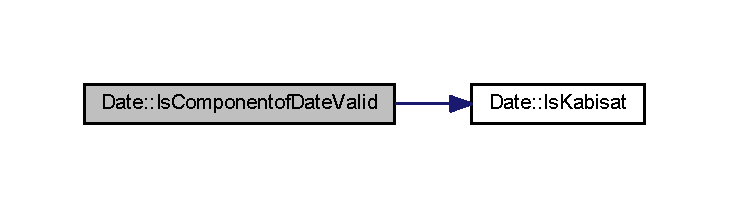
\includegraphics[width=350pt]{de/db5/class_date_a94fd42f78253556ad1e585ec473935b6_cgraph}
\end{center}
\end{figure}




Here is the caller graph for this function\-:\nopagebreak
\begin{figure}[H]
\begin{center}
\leavevmode
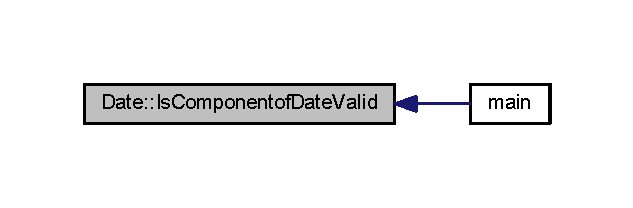
\includegraphics[width=304pt]{de/db5/class_date_a94fd42f78253556ad1e585ec473935b6_icgraph}
\end{center}
\end{figure}


\hypertarget{class_date_ae4cb2474b8a06d777264233188ed2720}{\index{Date@{Date}!Is\-Kabisat@{Is\-Kabisat}}
\index{Is\-Kabisat@{Is\-Kabisat}!Date@{Date}}
\subsubsection[{Is\-Kabisat}]{\setlength{\rightskip}{0pt plus 5cm}bool Date\-::\-Is\-Kabisat (
\begin{DoxyParamCaption}
\item[{const int \&}]{Year\-Component}
\end{DoxyParamCaption}
)\hspace{0.3cm}{\ttfamily [static]}}}\label{class_date_ae4cb2474b8a06d777264233188ed2720}


Determines if the year component of date is Kabisat or not. 

Year is Kabisat if Year can be divided by 4 but can't be divided by 100 or can be divided by 400


\begin{DoxyParams}[1]{Parameters}
\mbox{\tt in}  & {\em Year\-Component} & The year component of date. \\
\hline
\end{DoxyParams}
\begin{DoxyReturn}{Returns}
true if Year\-Component is kabisat; otherwise false. 
\end{DoxyReturn}


Definition at line 100 of file Date.\-cpp.



Here is the caller graph for this function\-:\nopagebreak
\begin{figure}[H]
\begin{center}
\leavevmode
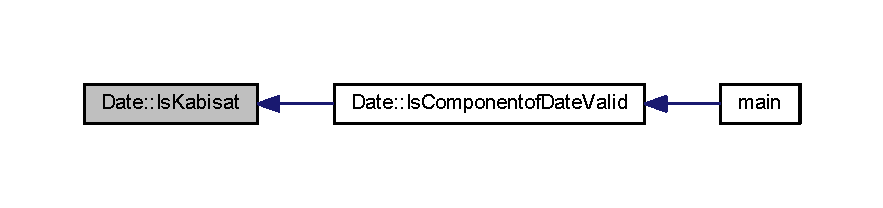
\includegraphics[width=350pt]{de/db5/class_date_ae4cb2474b8a06d777264233188ed2720_icgraph}
\end{center}
\end{figure}


\hypertarget{class_date_ae6e05500234df3028aace397f68b0929}{\index{Date@{Date}!operator!=@{operator!=}}
\index{operator!=@{operator!=}!Date@{Date}}
\subsubsection[{operator!=}]{\setlength{\rightskip}{0pt plus 5cm}bool Date\-::operator!= (
\begin{DoxyParamCaption}
\item[{const {\bf Date} \&}]{D}
\end{DoxyParamCaption}
)}}\label{class_date_ae6e05500234df3028aace397f68b0929}


Determines whether the specified object \hyperlink{class_date}{Date} is not equal to the current object \hyperlink{class_date}{Date}. 


\begin{DoxyParams}[1]{Parameters}
\mbox{\tt in}  & {\em D} & The object \hyperlink{class_date}{Date} to compare with the current object \hyperlink{class_date}{Date}. \\
\hline
\end{DoxyParams}
\begin{DoxyReturn}{Returns}
true if the specified \hyperlink{class_date}{Date} is not equal to the current \hyperlink{class_date}{Date}; otherwise false. 
\end{DoxyReturn}


Definition at line 31 of file Date.\-cpp.

\hypertarget{class_date_afb88829e04e94bbedb058aacfe6c9ab7}{\index{Date@{Date}!operator$<$@{operator$<$}}
\index{operator$<$@{operator$<$}!Date@{Date}}
\subsubsection[{operator$<$}]{\setlength{\rightskip}{0pt plus 5cm}bool Date\-::operator$<$ (
\begin{DoxyParamCaption}
\item[{const {\bf Date} \&}]{D}
\end{DoxyParamCaption}
)}}\label{class_date_afb88829e04e94bbedb058aacfe6c9ab7}


Determines whether the specified object \hyperlink{class_date}{Date} is earlier than the current object \hyperlink{class_date}{Date}. 


\begin{DoxyParams}[1]{Parameters}
\mbox{\tt in}  & {\em D} & The object \hyperlink{class_date}{Date} to compare with the current object \hyperlink{class_date}{Date}. \\
\hline
\end{DoxyParams}
\begin{DoxyReturn}{Returns}
true if the specified \hyperlink{class_date}{Date} is earlier to the current \hyperlink{class_date}{Date}; otherwise false. 
\end{DoxyReturn}


Definition at line 38 of file Date.\-cpp.

\hypertarget{class_date_adfb778e1afee2312a53597275e669ad6}{\index{Date@{Date}!operator==@{operator==}}
\index{operator==@{operator==}!Date@{Date}}
\subsubsection[{operator==}]{\setlength{\rightskip}{0pt plus 5cm}bool Date\-::operator== (
\begin{DoxyParamCaption}
\item[{const {\bf Date} \&}]{D}
\end{DoxyParamCaption}
)}}\label{class_date_adfb778e1afee2312a53597275e669ad6}


Determines whether the specified object \hyperlink{class_date}{Date} is equal to the current object \hyperlink{class_date}{Date}. 


\begin{DoxyParams}[1]{Parameters}
\mbox{\tt in}  & {\em D} & The object \hyperlink{class_date}{Date} to compare with the current object \hyperlink{class_date}{Date}. \\
\hline
\end{DoxyParams}
\begin{DoxyReturn}{Returns}
true if the specified \hyperlink{class_date}{Date} is equal to the current \hyperlink{class_date}{Date}; otherwise false. 
\end{DoxyReturn}


Definition at line 24 of file Date.\-cpp.

\hypertarget{class_date_a6e4731c11f54e00166edeb97b7e54037}{\index{Date@{Date}!operator$>$@{operator$>$}}
\index{operator$>$@{operator$>$}!Date@{Date}}
\subsubsection[{operator$>$}]{\setlength{\rightskip}{0pt plus 5cm}bool Date\-::operator$>$ (
\begin{DoxyParamCaption}
\item[{const {\bf Date} \&}]{D}
\end{DoxyParamCaption}
)}}\label{class_date_a6e4731c11f54e00166edeb97b7e54037}


Determines whether the specified object \hyperlink{class_date}{Date} is later than the current object \hyperlink{class_date}{Date}. 


\begin{DoxyParams}[1]{Parameters}
\mbox{\tt in}  & {\em D} & The object \hyperlink{class_date}{Date} to compare with the current object \hyperlink{class_date}{Date}. \\
\hline
\end{DoxyParams}
\begin{DoxyReturn}{Returns}
true if the specified \hyperlink{class_date}{Date} is later to the current \hyperlink{class_date}{Date}; otherwise false. 
\end{DoxyReturn}


Definition at line 51 of file Date.\-cpp.

\hypertarget{class_date_aa5ac806a5d140c3eb60e489f39b6ecdf}{\index{Date@{Date}!Set\-Dayof\-Date@{Set\-Dayof\-Date}}
\index{Set\-Dayof\-Date@{Set\-Dayof\-Date}!Date@{Date}}
\subsubsection[{Set\-Dayof\-Date}]{\setlength{\rightskip}{0pt plus 5cm}void Date\-::\-Set\-Dayof\-Date (
\begin{DoxyParamCaption}
\item[{int}]{Day\-Component}
\end{DoxyParamCaption}
)}}\label{class_date_aa5ac806a5d140c3eb60e489f39b6ecdf}


Set the day component of date with specified day. 

Parameter must be a valid Day\-Component


\begin{DoxyParams}[1]{Parameters}
\mbox{\tt in}  & {\em Day\-Component} & The new day component of date. \\
\hline
\end{DoxyParams}


Definition at line 125 of file Date.\-cpp.



Here is the caller graph for this function\-:\nopagebreak
\begin{figure}[H]
\begin{center}
\leavevmode
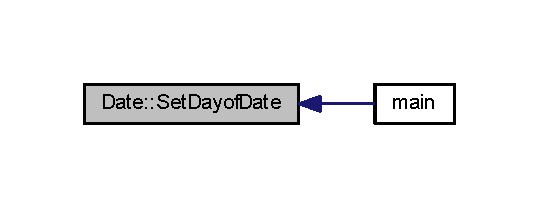
\includegraphics[width=258pt]{de/db5/class_date_aa5ac806a5d140c3eb60e489f39b6ecdf_icgraph}
\end{center}
\end{figure}


\hypertarget{class_date_a5c6fd52c67e4f09558fcbd788ed6fa55}{\index{Date@{Date}!Set\-Monthof\-Date@{Set\-Monthof\-Date}}
\index{Set\-Monthof\-Date@{Set\-Monthof\-Date}!Date@{Date}}
\subsubsection[{Set\-Monthof\-Date}]{\setlength{\rightskip}{0pt plus 5cm}void Date\-::\-Set\-Monthof\-Date (
\begin{DoxyParamCaption}
\item[{int}]{Month\-Component}
\end{DoxyParamCaption}
)}}\label{class_date_a5c6fd52c67e4f09558fcbd788ed6fa55}


Set the month component of date with specified month. 

Parameter must be a valid Month\-Component


\begin{DoxyParams}[1]{Parameters}
\mbox{\tt in}  & {\em Month\-Component} & The new month component of date. \\
\hline
\end{DoxyParams}


Definition at line 130 of file Date.\-cpp.



Here is the caller graph for this function\-:\nopagebreak
\begin{figure}[H]
\begin{center}
\leavevmode
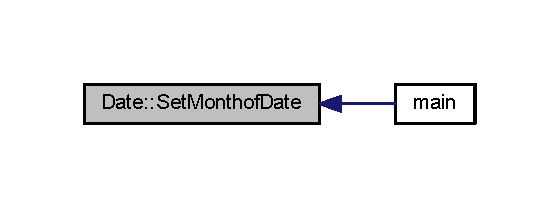
\includegraphics[width=268pt]{de/db5/class_date_a5c6fd52c67e4f09558fcbd788ed6fa55_icgraph}
\end{center}
\end{figure}


\hypertarget{class_date_a717961f3e2938f4b7e7523335b899cd6}{\index{Date@{Date}!Set\-Yearof\-Date@{Set\-Yearof\-Date}}
\index{Set\-Yearof\-Date@{Set\-Yearof\-Date}!Date@{Date}}
\subsubsection[{Set\-Yearof\-Date}]{\setlength{\rightskip}{0pt plus 5cm}void Date\-::\-Set\-Yearof\-Date (
\begin{DoxyParamCaption}
\item[{int}]{Year\-Component}
\end{DoxyParamCaption}
)}}\label{class_date_a717961f3e2938f4b7e7523335b899cd6}


Set the year component of date with specified year. 

Parameter must be a valid Year\-Component


\begin{DoxyParams}[1]{Parameters}
\mbox{\tt in}  & {\em Year\-Component} & The new year component of date. \\
\hline
\end{DoxyParams}


Definition at line 135 of file Date.\-cpp.



Here is the caller graph for this function\-:\nopagebreak
\begin{figure}[H]
\begin{center}
\leavevmode
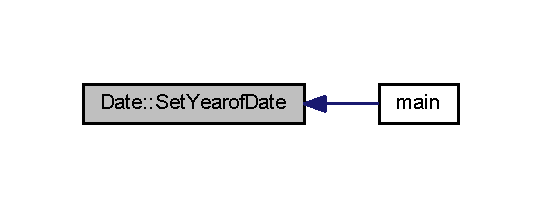
\includegraphics[width=260pt]{de/db5/class_date_a717961f3e2938f4b7e7523335b899cd6_icgraph}
\end{center}
\end{figure}




\subsection{Friends And Related Function Documentation}
\hypertarget{class_date_a9559c1c3841bdae17b284844a756d4bd}{\index{Date@{Date}!operator$<$$<$@{operator$<$$<$}}
\index{operator$<$$<$@{operator$<$$<$}!Date@{Date}}
\subsubsection[{operator$<$$<$}]{\setlength{\rightskip}{0pt plus 5cm}ostream\& operator$<$$<$ (
\begin{DoxyParamCaption}
\item[{ostream \&}]{output, }
\item[{const {\bf Date} \&}]{D}
\end{DoxyParamCaption}
)\hspace{0.3cm}{\ttfamily [friend]}}}\label{class_date_a9559c1c3841bdae17b284844a756d4bd}


Writes the specified \hyperlink{class_date}{Date} followed by the current line terminator to the standard output stream. 


\begin{DoxyParams}[1]{Parameters}
\mbox{\tt out}  & {\em output} & An instance of class ostream. \\
\hline
\mbox{\tt in}  & {\em D} & An instance of class \hyperlink{class_date}{Date}. \\
\hline
\end{DoxyParams}


Definition at line 108 of file Date.\-h.

\hypertarget{class_date_a8576024c4c197a313e26cd753347db6c}{\index{Date@{Date}!operator$>$$>$@{operator$>$$>$}}
\index{operator$>$$>$@{operator$>$$>$}!Date@{Date}}
\subsubsection[{operator$>$$>$}]{\setlength{\rightskip}{0pt plus 5cm}istream\& operator$>$$>$ (
\begin{DoxyParamCaption}
\item[{istream \&}]{input, }
\item[{{\bf Date} \&}]{D}
\end{DoxyParamCaption}
)\hspace{0.3cm}{\ttfamily [friend]}}}\label{class_date_a8576024c4c197a313e26cd753347db6c}


Read the specified \hyperlink{class_date}{Date} to the standard input stream. 


\begin{DoxyParams}[1]{Parameters}
\mbox{\tt out}  & {\em input} & An instance of class istream. \\
\hline
\mbox{\tt out}  & {\em D} & An instance of class \hyperlink{class_date}{Date}. \\
\hline
\end{DoxyParams}


Definition at line 86 of file Date.\-h.



The documentation for this class was generated from the following files\-:\begin{DoxyCompactItemize}
\item 
Date/\hyperlink{_date_8h}{Date.\-h}\item 
Date/\hyperlink{_date_8cpp}{Date.\-cpp}\end{DoxyCompactItemize}

\hypertarget{class_date_time}{\section{Date\-Time Class Reference}
\label{class_date_time}\index{Date\-Time@{Date\-Time}}
}


\hyperlink{class_date_time}{Date\-Time} Class.  




{\ttfamily \#include $<$Date\-Time.\-h$>$}

\subsection*{Public Member Functions}
\begin{DoxyCompactItemize}
\item 
\hyperlink{class_date_time_a5c46d6432c6df5d550603b529e825dc5}{$\sim$\-Date\-Time} ()
\begin{DoxyCompactList}\small\item\em Clear an instance of \hyperlink{class_date_time}{Date\-Time} from memory. \end{DoxyCompactList}\item 
bool \hyperlink{class_date_time_a61752bfcf9bfe5e2e9d493ac42fe3ee8}{operator==} (\hyperlink{class_date_time}{Date\-Time} D\-T)
\begin{DoxyCompactList}\small\item\em Determines whether the specified object \hyperlink{class_date_time}{Date\-Time} is equal to the current object \hyperlink{class_date_time}{Date\-Time}. \end{DoxyCompactList}\item 
bool \hyperlink{class_date_time_a6478a78407126774d91a631dedea5e84}{operator!=} (\hyperlink{class_date_time}{Date\-Time} D\-T)
\begin{DoxyCompactList}\small\item\em Determines whether the specified object \hyperlink{class_date_time}{Date\-Time} is not equal to the current object \hyperlink{class_date_time}{Date\-Time}. \end{DoxyCompactList}\item 
bool \hyperlink{class_date_time_a08f9db72e1d0f49916fe6686218402e8}{operator$<$} (\hyperlink{class_date_time}{Date\-Time} D\-T)
\begin{DoxyCompactList}\small\item\em Determines whether the specified object \hyperlink{class_date_time}{Date\-Time} is earlier than the current object \hyperlink{class_date_time}{Date\-Time}. \end{DoxyCompactList}\item 
bool \hyperlink{class_date_time_a0ebaa48c3c3c55751f3201c29379664e}{operator$>$} (\hyperlink{class_date_time}{Date\-Time} D\-T)
\begin{DoxyCompactList}\small\item\em Determines whether the specified object \hyperlink{class_date_time}{Date\-Time} is later than the current object \hyperlink{class_date_time}{Date\-Time}. \end{DoxyCompactList}\item 
\hyperlink{class_date}{Date} \hyperlink{class_date_time_a4c206227fdf530b862f4df46ee0da5b7}{Get\-Date} ()
\begin{DoxyCompactList}\small\item\em Gets the date from \hyperlink{class_date_time}{Date\-Time}. \end{DoxyCompactList}\item 
\hyperlink{class_time}{Time} \hyperlink{class_date_time_ab0b5363b639394082b8464107b96ef9c}{Get\-Time} ()
\begin{DoxyCompactList}\small\item\em Gets the time from \hyperlink{class_date_time}{Date\-Time}. \end{DoxyCompactList}\item 
void \hyperlink{class_date_time_af59006af64ac325b50d5d8c1dc6057b6}{Set\-Date} (\hyperlink{class_date}{Date} \hyperlink{class_date}{Date})
\begin{DoxyCompactList}\small\item\em Set the \hyperlink{class_date}{Date} of \hyperlink{class_date_time}{Date\-Time} with specified \hyperlink{class_date}{Date}. \end{DoxyCompactList}\item 
void \hyperlink{class_date_time_a59940dc8f5f4f7d938e2bdbe3b68eba2}{Set\-Time} (\hyperlink{class_time}{Time} \hyperlink{class_time}{Time})
\begin{DoxyCompactList}\small\item\em Set the \hyperlink{class_time}{Time} of \hyperlink{class_date_time}{Date\-Time} with specified \hyperlink{class_time}{Time}. \end{DoxyCompactList}\end{DoxyCompactItemize}
\subsection*{Friends}
\begin{DoxyCompactItemize}
\item 
istream \& \hyperlink{class_date_time_a2a7b5a6ce0f12397e2fc83060106cfbd}{operator$>$$>$} (istream \&input, \hyperlink{class_date_time}{Date\-Time} \&D\-T)
\begin{DoxyCompactList}\small\item\em Read the specified \hyperlink{class_date_time}{Date\-Time} to the standard input stream. \end{DoxyCompactList}\item 
ostream \& \hyperlink{class_date_time_aaffa9ef1d2a2e41e2e2765dbcbfdcdae}{operator$<$$<$} (ostream \&output, const \hyperlink{class_date_time}{Date\-Time} \&D\-T)
\begin{DoxyCompactList}\small\item\em Writes the specified \hyperlink{class_date_time}{Date\-Time} followed by the current line terminator to the standard output stream. \end{DoxyCompactList}\end{DoxyCompactItemize}
\subsection*{Related Functions}
(Note that these are not member functions.) \begin{DoxyCompactItemize}
\item 
\hyperlink{class_date_time_a3ccfb87f7a2e9683b91964e32d907161}{Date\-Time} ()
\begin{DoxyCompactList}\small\item\em Initializes a new instance of the \hyperlink{class_date_time}{Date\-Time} class. \end{DoxyCompactList}\item 
\hyperlink{class_date_time_a68fb98c071f90a98561c3b33737f9600}{Date\-Time} (const \hyperlink{class_date_time}{Date\-Time} \&D\-T)
\begin{DoxyCompactList}\small\item\em Initializes a new instance of the \hyperlink{class_date_time}{Date\-Time} class from specified \hyperlink{class_date_time}{Date\-Time}. \end{DoxyCompactList}\end{DoxyCompactItemize}


\subsection{Detailed Description}
\hyperlink{class_date_time}{Date\-Time} Class. 

Represent \hyperlink{class_date}{Date} and \hyperlink{class_time}{Time}

\begin{DoxyNote}{Note}
Use \hyperlink{class_date}{Date} and \hyperlink{class_time}{Time} Class
\end{DoxyNote}
\begin{DoxyAuthor}{Author}
Riva Syafri Rachmatullah (13512036) for .h file 

Indam Muhammad (13512036) and Riva Syafri Rachmatullah (13512036) for .cpp file
\end{DoxyAuthor}
\begin{DoxyVersion}{Version}
v1.\-3 
\end{DoxyVersion}


Definition at line 30 of file Date\-Time.\-h.



\subsection{Constructor \& Destructor Documentation}
\hypertarget{class_date_time_a5c46d6432c6df5d550603b529e825dc5}{\index{Date\-Time@{Date\-Time}!$\sim$\-Date\-Time@{$\sim$\-Date\-Time}}
\index{$\sim$\-Date\-Time@{$\sim$\-Date\-Time}!DateTime@{Date\-Time}}
\subsubsection[{$\sim$\-Date\-Time}]{\setlength{\rightskip}{0pt plus 5cm}Date\-Time\-::$\sim$\-Date\-Time (
\begin{DoxyParamCaption}
{}
\end{DoxyParamCaption}
)}}\label{class_date_time_a5c46d6432c6df5d550603b529e825dc5}


Clear an instance of \hyperlink{class_date_time}{Date\-Time} from memory. 



Definition at line 19 of file Date\-Time.\-cpp.



\subsection{Member Function Documentation}
\hypertarget{class_date_time_a4c206227fdf530b862f4df46ee0da5b7}{\index{Date\-Time@{Date\-Time}!Get\-Date@{Get\-Date}}
\index{Get\-Date@{Get\-Date}!DateTime@{Date\-Time}}
\subsubsection[{Get\-Date}]{\setlength{\rightskip}{0pt plus 5cm}{\bf Date} Date\-Time\-::\-Get\-Date (
\begin{DoxyParamCaption}
{}
\end{DoxyParamCaption}
)}}\label{class_date_time_a4c206227fdf530b862f4df46ee0da5b7}


Gets the date from \hyperlink{class_date_time}{Date\-Time}. 

\begin{DoxyReturn}{Returns}
The time from \hyperlink{class_date_time}{Date\-Time}. 
\end{DoxyReturn}


Definition at line 49 of file Date\-Time.\-cpp.

\hypertarget{class_date_time_ab0b5363b639394082b8464107b96ef9c}{\index{Date\-Time@{Date\-Time}!Get\-Time@{Get\-Time}}
\index{Get\-Time@{Get\-Time}!DateTime@{Date\-Time}}
\subsubsection[{Get\-Time}]{\setlength{\rightskip}{0pt plus 5cm}{\bf Time} Date\-Time\-::\-Get\-Time (
\begin{DoxyParamCaption}
{}
\end{DoxyParamCaption}
)}}\label{class_date_time_ab0b5363b639394082b8464107b96ef9c}


Gets the time from \hyperlink{class_date_time}{Date\-Time}. 

\begin{DoxyReturn}{Returns}
The time from \hyperlink{class_date_time}{Date\-Time}. 
\end{DoxyReturn}


Definition at line 54 of file Date\-Time.\-cpp.

\hypertarget{class_date_time_a6478a78407126774d91a631dedea5e84}{\index{Date\-Time@{Date\-Time}!operator!=@{operator!=}}
\index{operator!=@{operator!=}!DateTime@{Date\-Time}}
\subsubsection[{operator!=}]{\setlength{\rightskip}{0pt plus 5cm}bool Date\-Time\-::operator!= (
\begin{DoxyParamCaption}
\item[{{\bf Date\-Time}}]{D\-T}
\end{DoxyParamCaption}
)}}\label{class_date_time_a6478a78407126774d91a631dedea5e84}


Determines whether the specified object \hyperlink{class_date_time}{Date\-Time} is not equal to the current object \hyperlink{class_date_time}{Date\-Time}. 


\begin{DoxyParams}[1]{Parameters}
\mbox{\tt in}  & {\em D\-T} & The object \hyperlink{class_date_time}{Date\-Time} to compare with the current object \hyperlink{class_date_time}{Date\-Time}. \\
\hline
\end{DoxyParams}
\begin{DoxyReturn}{Returns}
true if the specified object \hyperlink{class_date_time}{Date\-Time} is not equal to the current object \hyperlink{class_date_time}{Date\-Time}; otherwise false. 
\end{DoxyReturn}


Definition at line 27 of file Date\-Time.\-cpp.

\hypertarget{class_date_time_a08f9db72e1d0f49916fe6686218402e8}{\index{Date\-Time@{Date\-Time}!operator$<$@{operator$<$}}
\index{operator$<$@{operator$<$}!DateTime@{Date\-Time}}
\subsubsection[{operator$<$}]{\setlength{\rightskip}{0pt plus 5cm}bool Date\-Time\-::operator$<$ (
\begin{DoxyParamCaption}
\item[{{\bf Date\-Time}}]{D\-T}
\end{DoxyParamCaption}
)}}\label{class_date_time_a08f9db72e1d0f49916fe6686218402e8}


Determines whether the specified object \hyperlink{class_date_time}{Date\-Time} is earlier than the current object \hyperlink{class_date_time}{Date\-Time}. 


\begin{DoxyParams}[1]{Parameters}
\mbox{\tt in}  & {\em D\-T} & The object \hyperlink{class_date_time}{Date\-Time} to compare with the current object \hyperlink{class_date_time}{Date\-Time}. \\
\hline
\end{DoxyParams}
\begin{DoxyReturn}{Returns}
true if the specified object \hyperlink{class_date_time}{Date\-Time} is earlier than to the current object \hyperlink{class_date_time}{Date\-Time}; otherwise false. 
\end{DoxyReturn}


Definition at line 33 of file Date\-Time.\-cpp.

\hypertarget{class_date_time_a61752bfcf9bfe5e2e9d493ac42fe3ee8}{\index{Date\-Time@{Date\-Time}!operator==@{operator==}}
\index{operator==@{operator==}!DateTime@{Date\-Time}}
\subsubsection[{operator==}]{\setlength{\rightskip}{0pt plus 5cm}bool Date\-Time\-::operator== (
\begin{DoxyParamCaption}
\item[{{\bf Date\-Time}}]{D\-T}
\end{DoxyParamCaption}
)}}\label{class_date_time_a61752bfcf9bfe5e2e9d493ac42fe3ee8}


Determines whether the specified object \hyperlink{class_date_time}{Date\-Time} is equal to the current object \hyperlink{class_date_time}{Date\-Time}. 


\begin{DoxyParams}[1]{Parameters}
\mbox{\tt in}  & {\em D\-T} & The object \hyperlink{class_date_time}{Date\-Time} to compare with the current object \hyperlink{class_date_time}{Date\-Time}. \\
\hline
\end{DoxyParams}
\begin{DoxyReturn}{Returns}
true if the specified object \hyperlink{class_date_time}{Date\-Time} is equal to the current object \hyperlink{class_date_time}{Date\-Time}; otherwise false. 
\end{DoxyReturn}


Definition at line 21 of file Date\-Time.\-cpp.

\hypertarget{class_date_time_a0ebaa48c3c3c55751f3201c29379664e}{\index{Date\-Time@{Date\-Time}!operator$>$@{operator$>$}}
\index{operator$>$@{operator$>$}!DateTime@{Date\-Time}}
\subsubsection[{operator$>$}]{\setlength{\rightskip}{0pt plus 5cm}bool Date\-Time\-::operator$>$ (
\begin{DoxyParamCaption}
\item[{{\bf Date\-Time}}]{D\-T}
\end{DoxyParamCaption}
)}}\label{class_date_time_a0ebaa48c3c3c55751f3201c29379664e}


Determines whether the specified object \hyperlink{class_date_time}{Date\-Time} is later than the current object \hyperlink{class_date_time}{Date\-Time}. 


\begin{DoxyParams}[1]{Parameters}
\mbox{\tt in}  & {\em D\-T} & The object \hyperlink{class_date_time}{Date\-Time} to compare with the current object \hyperlink{class_date_time}{Date\-Time}. \\
\hline
\end{DoxyParams}
\begin{DoxyReturn}{Returns}
true if the specified object \hyperlink{class_date_time}{Date\-Time} is later than to the current object \hyperlink{class_date_time}{Date\-Time}; otherwise false. 
\end{DoxyReturn}


Definition at line 41 of file Date\-Time.\-cpp.

\hypertarget{class_date_time_af59006af64ac325b50d5d8c1dc6057b6}{\index{Date\-Time@{Date\-Time}!Set\-Date@{Set\-Date}}
\index{Set\-Date@{Set\-Date}!DateTime@{Date\-Time}}
\subsubsection[{Set\-Date}]{\setlength{\rightskip}{0pt plus 5cm}void Date\-Time\-::\-Set\-Date (
\begin{DoxyParamCaption}
\item[{{\bf Date}}]{Date}
\end{DoxyParamCaption}
)}}\label{class_date_time_af59006af64ac325b50d5d8c1dc6057b6}


Set the \hyperlink{class_date}{Date} of \hyperlink{class_date_time}{Date\-Time} with specified \hyperlink{class_date}{Date}. 


\begin{DoxyParams}[1]{Parameters}
\mbox{\tt in}  & {\em \hyperlink{class_date}{Date}} & The new \hyperlink{class_date}{Date} of \hyperlink{class_date_time}{Date\-Time}. \\
\hline
\end{DoxyParams}


Definition at line 58 of file Date\-Time.\-cpp.



Here is the caller graph for this function\-:\nopagebreak
\begin{figure}[H]
\begin{center}
\leavevmode
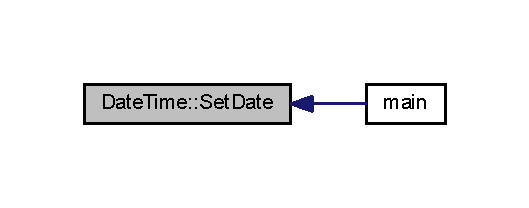
\includegraphics[width=254pt]{d7/d85/class_date_time_af59006af64ac325b50d5d8c1dc6057b6_icgraph}
\end{center}
\end{figure}


\hypertarget{class_date_time_a59940dc8f5f4f7d938e2bdbe3b68eba2}{\index{Date\-Time@{Date\-Time}!Set\-Time@{Set\-Time}}
\index{Set\-Time@{Set\-Time}!DateTime@{Date\-Time}}
\subsubsection[{Set\-Time}]{\setlength{\rightskip}{0pt plus 5cm}void Date\-Time\-::\-Set\-Time (
\begin{DoxyParamCaption}
\item[{{\bf Time}}]{Time}
\end{DoxyParamCaption}
)}}\label{class_date_time_a59940dc8f5f4f7d938e2bdbe3b68eba2}


Set the \hyperlink{class_time}{Time} of \hyperlink{class_date_time}{Date\-Time} with specified \hyperlink{class_time}{Time}. 


\begin{DoxyParams}[1]{Parameters}
\mbox{\tt in}  & {\em \hyperlink{class_time}{Time}} & The new \hyperlink{class_time}{Time} of \hyperlink{class_date_time}{Date\-Time}. \\
\hline
\end{DoxyParams}


Definition at line 62 of file Date\-Time.\-cpp.



Here is the caller graph for this function\-:\nopagebreak
\begin{figure}[H]
\begin{center}
\leavevmode
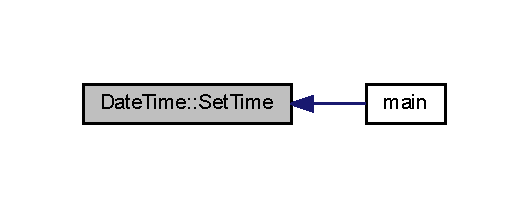
\includegraphics[width=254pt]{d7/d85/class_date_time_a59940dc8f5f4f7d938e2bdbe3b68eba2_icgraph}
\end{center}
\end{figure}




\subsection{Friends And Related Function Documentation}
\hypertarget{class_date_time_a3ccfb87f7a2e9683b91964e32d907161}{\index{Date\-Time@{Date\-Time}!Date\-Time@{Date\-Time}}
\index{Date\-Time@{Date\-Time}!DateTime@{Date\-Time}}
\subsubsection[{Date\-Time}]{\setlength{\rightskip}{0pt plus 5cm}Date\-Time\-::\-Date\-Time (
\begin{DoxyParamCaption}
{}
\end{DoxyParamCaption}
)\hspace{0.3cm}{\ttfamily [related]}}}\label{class_date_time_a3ccfb87f7a2e9683b91964e32d907161}


Initializes a new instance of the \hyperlink{class_date_time}{Date\-Time} class. 



Definition at line 11 of file Date\-Time.\-cpp.

\hypertarget{class_date_time_a68fb98c071f90a98561c3b33737f9600}{\index{Date\-Time@{Date\-Time}!Date\-Time@{Date\-Time}}
\index{Date\-Time@{Date\-Time}!DateTime@{Date\-Time}}
\subsubsection[{Date\-Time}]{\setlength{\rightskip}{0pt plus 5cm}Date\-Time\-::\-Date\-Time (
\begin{DoxyParamCaption}
\item[{const {\bf Date\-Time} \&}]{D\-T}
\end{DoxyParamCaption}
)\hspace{0.3cm}{\ttfamily [related]}}}\label{class_date_time_a68fb98c071f90a98561c3b33737f9600}


Initializes a new instance of the \hyperlink{class_date_time}{Date\-Time} class from specified \hyperlink{class_date_time}{Date\-Time}. 


\begin{DoxyParams}[1]{Parameters}
\mbox{\tt in}  & {\em D\-T} & The object \hyperlink{class_date_time}{Date\-Time} that will be copied. \\
\hline
\end{DoxyParams}


Definition at line 13 of file Date\-Time.\-cpp.

\hypertarget{class_date_time_aaffa9ef1d2a2e41e2e2765dbcbfdcdae}{\index{Date\-Time@{Date\-Time}!operator$<$$<$@{operator$<$$<$}}
\index{operator$<$$<$@{operator$<$$<$}!DateTime@{Date\-Time}}
\subsubsection[{operator$<$$<$}]{\setlength{\rightskip}{0pt plus 5cm}ostream\& operator$<$$<$ (
\begin{DoxyParamCaption}
\item[{ostream \&}]{output, }
\item[{const {\bf Date\-Time} \&}]{D\-T}
\end{DoxyParamCaption}
)\hspace{0.3cm}{\ttfamily [friend]}}}\label{class_date_time_aaffa9ef1d2a2e41e2e2765dbcbfdcdae}


Writes the specified \hyperlink{class_date_time}{Date\-Time} followed by the current line terminator to the standard output stream. 


\begin{DoxyParams}[1]{Parameters}
\mbox{\tt out}  & {\em output} & An instance of class ostream. \\
\hline
\mbox{\tt in}  & {\em D\-T} & An instance of class \hyperlink{class_date_time}{Date\-Time}. \\
\hline
\end{DoxyParams}


Definition at line 122 of file Date\-Time.\-h.

\hypertarget{class_date_time_a2a7b5a6ce0f12397e2fc83060106cfbd}{\index{Date\-Time@{Date\-Time}!operator$>$$>$@{operator$>$$>$}}
\index{operator$>$$>$@{operator$>$$>$}!DateTime@{Date\-Time}}
\subsubsection[{operator$>$$>$}]{\setlength{\rightskip}{0pt plus 5cm}istream\& operator$>$$>$ (
\begin{DoxyParamCaption}
\item[{istream \&}]{input, }
\item[{{\bf Date\-Time} \&}]{D\-T}
\end{DoxyParamCaption}
)\hspace{0.3cm}{\ttfamily [friend]}}}\label{class_date_time_a2a7b5a6ce0f12397e2fc83060106cfbd}


Read the specified \hyperlink{class_date_time}{Date\-Time} to the standard input stream. 


\begin{DoxyParams}[1]{Parameters}
\mbox{\tt out}  & {\em input} & An instance of class istream. \\
\hline
\mbox{\tt out}  & {\em D\-T} & An instance of class \hyperlink{class_date_time}{Date\-Time}. \\
\hline
\end{DoxyParams}


Definition at line 96 of file Date\-Time.\-h.



The documentation for this class was generated from the following files\-:\begin{DoxyCompactItemize}
\item 
Date\-Time/\hyperlink{_date_time_8h}{Date\-Time.\-h}\item 
Date\-Time/\hyperlink{_date_time_8cpp}{Date\-Time.\-cpp}\end{DoxyCompactItemize}

\hypertarget{class_event}{\section{Event Class Reference}
\label{class_event}\index{Event@{Event}}
}


\hyperlink{class_event}{Event} Class.  




{\ttfamily \#include $<$Event.\-h$>$}

\subsection*{Public Member Functions}
\begin{DoxyCompactItemize}
\item 
\hyperlink{class_event_a7704ec01ce91e673885792054214b3d2}{$\sim$\-Event} ()
\begin{DoxyCompactList}\small\item\em Clear an instance of \hyperlink{class_event}{Event} from memory. \end{DoxyCompactList}\item 
\hyperlink{class_date_time}{Date\-Time} \hyperlink{class_event_ab828b0511da4f76c3090c88d8c9bbe2c}{Get\-Date\-Time} ()
\begin{DoxyCompactList}\small\item\em Gets \hyperlink{class_date_time}{Date\-Time} on an instance \hyperlink{class_event}{Event}. \end{DoxyCompactList}\item 
\hyperlink{class_date_time}{Date\-Time} \hyperlink{class_event_aeaea78f235bea3fc083f1a070c7e821a}{Get\-Deadline} ()
\begin{DoxyCompactList}\small\item\em Gets Deadline on an instance \hyperlink{class_event}{Event}. \end{DoxyCompactList}\item 
void \hyperlink{class_event_a70a345abe7ed4136058524ffdf3d3d53}{Set\-Deadline} (\hyperlink{class_date_time}{Date\-Time} Deadline)
\begin{DoxyCompactList}\small\item\em Set Deadline on \hyperlink{class_event}{Event}. \end{DoxyCompactList}\item 
void \hyperlink{class_event_acc0755128d9534def434679355004e79}{Close} ()
\begin{DoxyCompactList}\small\item\em Clear all the \hyperlink{class_teller}{Teller}. \end{DoxyCompactList}\end{DoxyCompactItemize}
\subsection*{Friends}
\begin{DoxyCompactItemize}
\item 
istream \& \hyperlink{class_event_aefab4a45e8de8a212980527a504d6061}{operator$>$$>$} (istream \&input, \hyperlink{class_event}{Event} \&E)
\begin{DoxyCompactList}\small\item\em Read the specified \hyperlink{class_event}{Event} to the standard input stream. \end{DoxyCompactList}\end{DoxyCompactItemize}
\subsection*{Related Functions}
(Note that these are not member functions.) \begin{DoxyCompactItemize}
\item 
\hyperlink{class_event_a5a40dd4708297f7031e29b39e039ae10}{Event} ()
\begin{DoxyCompactList}\small\item\em Initializes a new instance of the \hyperlink{class_event}{Event} class with 5 \hyperlink{class_teller}{Teller}. \end{DoxyCompactList}\item 
\hyperlink{class_event_a0cb91170821c7766ba1a142f80c1816e}{Event} (int Numberof\-Teller)
\begin{DoxyCompactList}\small\item\em Initializes a new instance of the \hyperlink{class_event}{Event} class with specified amount of \hyperlink{class_teller}{Teller}. \end{DoxyCompactList}\end{DoxyCompactItemize}


\subsection{Detailed Description}
\hyperlink{class_event}{Event} Class. 

Represent a \hyperlink{class_event}{Event}

\begin{DoxyAuthor}{Author}
Riva Syafri Rachmatullah (13512036) for .h file 

Riva Syafri Rachmatullah (13512036) for .cpp file
\end{DoxyAuthor}
\begin{DoxyVersion}{Version}
v1.\-2 
\end{DoxyVersion}


Definition at line 27 of file Event.\-h.



\subsection{Constructor \& Destructor Documentation}
\hypertarget{class_event_a7704ec01ce91e673885792054214b3d2}{\index{Event@{Event}!$\sim$\-Event@{$\sim$\-Event}}
\index{$\sim$\-Event@{$\sim$\-Event}!Event@{Event}}
\subsubsection[{$\sim$\-Event}]{\setlength{\rightskip}{0pt plus 5cm}Event\-::$\sim$\-Event (
\begin{DoxyParamCaption}
{}
\end{DoxyParamCaption}
)}}\label{class_event_a7704ec01ce91e673885792054214b3d2}


Clear an instance of \hyperlink{class_event}{Event} from memory. 



Definition at line 18 of file Event.\-cpp.



\subsection{Member Function Documentation}
\hypertarget{class_event_acc0755128d9534def434679355004e79}{\index{Event@{Event}!Close@{Close}}
\index{Close@{Close}!Event@{Event}}
\subsubsection[{Close}]{\setlength{\rightskip}{0pt plus 5cm}void Event\-::\-Close (
\begin{DoxyParamCaption}
{}
\end{DoxyParamCaption}
)}}\label{class_event_acc0755128d9534def434679355004e79}


Clear all the \hyperlink{class_teller}{Teller}. 

Each of teller will delete an element and print it. 

Definition at line 34 of file Event.\-cpp.



Here is the call graph for this function\-:\nopagebreak
\begin{figure}[H]
\begin{center}
\leavevmode
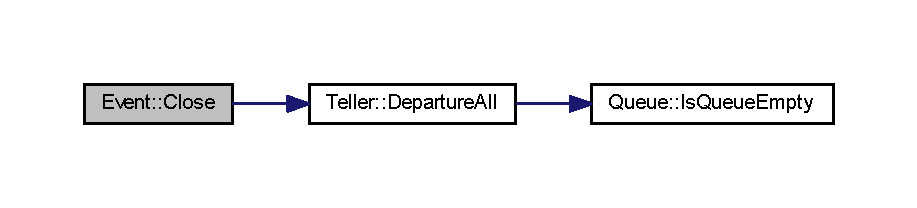
\includegraphics[width=350pt]{d1/da9/class_event_acc0755128d9534def434679355004e79_cgraph}
\end{center}
\end{figure}




Here is the caller graph for this function\-:\nopagebreak
\begin{figure}[H]
\begin{center}
\leavevmode
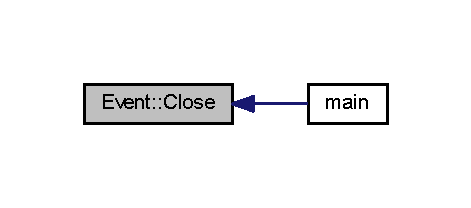
\includegraphics[width=226pt]{d1/da9/class_event_acc0755128d9534def434679355004e79_icgraph}
\end{center}
\end{figure}


\hypertarget{class_event_ab828b0511da4f76c3090c88d8c9bbe2c}{\index{Event@{Event}!Get\-Date\-Time@{Get\-Date\-Time}}
\index{Get\-Date\-Time@{Get\-Date\-Time}!Event@{Event}}
\subsubsection[{Get\-Date\-Time}]{\setlength{\rightskip}{0pt plus 5cm}{\bf Date\-Time} Event\-::\-Get\-Date\-Time (
\begin{DoxyParamCaption}
{}
\end{DoxyParamCaption}
)}}\label{class_event_ab828b0511da4f76c3090c88d8c9bbe2c}


Gets \hyperlink{class_date_time}{Date\-Time} on an instance \hyperlink{class_event}{Event}. 

\begin{DoxyReturn}{Returns}
\hyperlink{class_date_time}{Date\-Time} of \hyperlink{class_event}{Event}. 
\end{DoxyReturn}


Definition at line 22 of file Event.\-cpp.

\hypertarget{class_event_aeaea78f235bea3fc083f1a070c7e821a}{\index{Event@{Event}!Get\-Deadline@{Get\-Deadline}}
\index{Get\-Deadline@{Get\-Deadline}!Event@{Event}}
\subsubsection[{Get\-Deadline}]{\setlength{\rightskip}{0pt plus 5cm}{\bf Date\-Time} Event\-::\-Get\-Deadline (
\begin{DoxyParamCaption}
{}
\end{DoxyParamCaption}
)}}\label{class_event_aeaea78f235bea3fc083f1a070c7e821a}


Gets Deadline on an instance \hyperlink{class_event}{Event}. 

\begin{DoxyReturn}{Returns}
Deadline of \hyperlink{class_event}{Event}. 
\end{DoxyReturn}


Definition at line 26 of file Event.\-cpp.

\hypertarget{class_event_a70a345abe7ed4136058524ffdf3d3d53}{\index{Event@{Event}!Set\-Deadline@{Set\-Deadline}}
\index{Set\-Deadline@{Set\-Deadline}!Event@{Event}}
\subsubsection[{Set\-Deadline}]{\setlength{\rightskip}{0pt plus 5cm}void Event\-::\-Set\-Deadline (
\begin{DoxyParamCaption}
\item[{{\bf Date\-Time}}]{Deadline}
\end{DoxyParamCaption}
)}}\label{class_event_a70a345abe7ed4136058524ffdf3d3d53}


Set Deadline on \hyperlink{class_event}{Event}. 


\begin{DoxyParams}[1]{Parameters}
\mbox{\tt in}  & {\em Deadline} & The \hyperlink{class_date_time}{Date\-Time} for a Deadline of \hyperlink{class_event}{Event}. \\
\hline
\end{DoxyParams}


Definition at line 30 of file Event.\-cpp.



Here is the caller graph for this function\-:\nopagebreak
\begin{figure}[H]
\begin{center}
\leavevmode
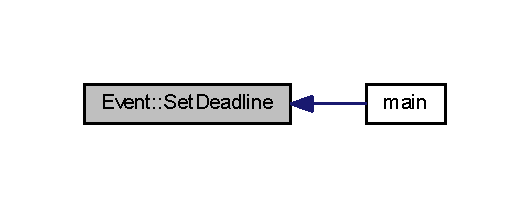
\includegraphics[width=254pt]{d1/da9/class_event_a70a345abe7ed4136058524ffdf3d3d53_icgraph}
\end{center}
\end{figure}




\subsection{Friends And Related Function Documentation}
\hypertarget{class_event_a5a40dd4708297f7031e29b39e039ae10}{\index{Event@{Event}!Event@{Event}}
\index{Event@{Event}!Event@{Event}}
\subsubsection[{Event}]{\setlength{\rightskip}{0pt plus 5cm}Event\-::\-Event (
\begin{DoxyParamCaption}
{}
\end{DoxyParamCaption}
)\hspace{0.3cm}{\ttfamily [related]}}}\label{class_event_a5a40dd4708297f7031e29b39e039ae10}


Initializes a new instance of the \hyperlink{class_event}{Event} class with 5 \hyperlink{class_teller}{Teller}. 



Definition at line 10 of file Event.\-cpp.

\hypertarget{class_event_a0cb91170821c7766ba1a142f80c1816e}{\index{Event@{Event}!Event@{Event}}
\index{Event@{Event}!Event@{Event}}
\subsubsection[{Event}]{\setlength{\rightskip}{0pt plus 5cm}Event\-::\-Event (
\begin{DoxyParamCaption}
\item[{int}]{Numberof\-Teller}
\end{DoxyParamCaption}
)\hspace{0.3cm}{\ttfamily [related]}}}\label{class_event_a0cb91170821c7766ba1a142f80c1816e}


Initializes a new instance of the \hyperlink{class_event}{Event} class with specified amount of \hyperlink{class_teller}{Teller}. 


\begin{DoxyParams}[1]{Parameters}
\mbox{\tt in}  & {\em Numberof\-Teller} & Amount of \hyperlink{class_teller}{Teller}. \\
\hline
\end{DoxyParams}


Definition at line 14 of file Event.\-cpp.

\hypertarget{class_event_aefab4a45e8de8a212980527a504d6061}{\index{Event@{Event}!operator$>$$>$@{operator$>$$>$}}
\index{operator$>$$>$@{operator$>$$>$}!Event@{Event}}
\subsubsection[{operator$>$$>$}]{\setlength{\rightskip}{0pt plus 5cm}istream\& operator$>$$>$ (
\begin{DoxyParamCaption}
\item[{istream \&}]{input, }
\item[{{\bf Event} \&}]{E}
\end{DoxyParamCaption}
)\hspace{0.3cm}{\ttfamily [friend]}}}\label{class_event_aefab4a45e8de8a212980527a504d6061}


Read the specified \hyperlink{class_event}{Event} to the standard input stream. 


\begin{DoxyParams}[1]{Parameters}
\mbox{\tt out}  & {\em input} & An instance of class istream. \\
\hline
\mbox{\tt out}  & {\em E} & An instance of class \hyperlink{class_event}{Event}. \\
\hline
\end{DoxyParams}


Definition at line 61 of file Event.\-h.



The documentation for this class was generated from the following files\-:\begin{DoxyCompactItemize}
\item 
Event/\hyperlink{_event_8h}{Event.\-h}\item 
Event/\hyperlink{_event_8cpp}{Event.\-cpp}\end{DoxyCompactItemize}

\hypertarget{class_queue}{\section{Queue Class Reference}
\label{class_queue}\index{Queue@{Queue}}
}


\hyperlink{class_queue}{Queue} Class.  




{\ttfamily \#include $<$Queue.\-h$>$}

\subsection*{Public Member Functions}
\begin{DoxyCompactItemize}
\item 
\hyperlink{class_queue_a7cfca3637d57c4a9e37351b3426ffd40}{Queue} ()
\begin{DoxyCompactList}\small\item\em Initializes a new instance of the \hyperlink{class_queue}{Queue} class with 26 block of memory. \end{DoxyCompactList}\item 
\hyperlink{class_queue_a9477bb38927e458bb211eb99cf89bda4}{Queue} (int Maximum\-Capacityof\-Queue)
\begin{DoxyCompactList}\small\item\em Initializes a new instance of the \hyperlink{class_queue}{Queue} class with Maximum\-Elementof\-Queue + 1 block of memory. \end{DoxyCompactList}\item 
\hyperlink{class_queue_acc9bf68f03677ae4e23dfda08f6ab63a}{Queue} (const \hyperlink{class_queue}{Queue} \&Q)
\begin{DoxyCompactList}\small\item\em Initializes a new instance of the \hyperlink{class_queue}{Queue} class with all the content of specified \hyperlink{class_queue}{Queue}. \end{DoxyCompactList}\item 
\hyperlink{class_queue}{Queue} \& \hyperlink{class_queue_a924ed23e355678aabd5d80551e9d3800}{operator=} (const \hyperlink{class_queue}{Queue} \&Q)
\begin{DoxyCompactList}\small\item\em Copy all content of specified \hyperlink{class_queue}{Queue} to current \hyperlink{class_queue}{Queue}. \end{DoxyCompactList}\item 
\hyperlink{class_queue_a00d119db8fa3050da37746e82cbcf94f}{$\sim$\-Queue} ()
\begin{DoxyCompactList}\small\item\em Clear an instance of \hyperlink{class_queue}{Queue} from memory. \end{DoxyCompactList}\item 
int \hyperlink{class_queue_a087160b0386fe1fdc7a0217fc40e4c94}{Addressof\-Head} ()
\begin{DoxyCompactList}\small\item\em Gets the Head address of queue. \end{DoxyCompactList}\item 
int \hyperlink{class_queue_ae9c7db696b3a50729b339ced74e0887a}{Addressof\-Tail} ()
\begin{DoxyCompactList}\small\item\em Gets the Tail address of queue. \end{DoxyCompactList}\item 
int \hyperlink{class_queue_ac3aa4048853f51c0552d532036b31cd6}{Contentof\-Head} ()
\begin{DoxyCompactList}\small\item\em Gets the content on \hyperlink{class_queue}{Queue}'s Head address. 
\begin{DoxyExceptions}{Exceptions}
{\em Invalid\-Operation\-Exception} & \hyperlink{class_queue}{Queue} is empty. \\
\hline
\end{DoxyExceptions}
\end{DoxyCompactList}\item 
int \hyperlink{class_queue_a019423c548927a8830677d1d2fddb38c}{Contentof\-Tail} ()
\begin{DoxyCompactList}\small\item\em Gets the content on \hyperlink{class_queue}{Queue}'s Tail address. 
\begin{DoxyExceptions}{Exceptions}
{\em Invalid\-Operation\-Exception} & \hyperlink{class_queue}{Queue} is empty. \\
\hline
\end{DoxyExceptions}
\end{DoxyCompactList}\item 
int \hyperlink{class_queue_a2b28fe3446577261546f74b7bbe3ccc6}{Size} ()
\begin{DoxyCompactList}\small\item\em Gets the maximum capacity that can be stored on \hyperlink{class_queue}{Queue}. \end{DoxyCompactList}\item 
bool \hyperlink{class_queue_abb997d38f5ac3bb506d8d073289affc1}{Is\-Queue\-Empty} ()
\begin{DoxyCompactList}\small\item\em Determines whether \hyperlink{class_queue}{Queue} is empty or not. \end{DoxyCompactList}\item 
bool \hyperlink{class_queue_a2815639bf7c03ea9ccda9fa30c20f52e}{Is\-Queue\-Full} ()
\begin{DoxyCompactList}\small\item\em Determines whether \hyperlink{class_queue}{Queue} is full or not. \end{DoxyCompactList}\item 
int \hyperlink{class_queue_ab9e0ba7176e94e7ee0ef75f0ef6120b0}{Effective} ()
\begin{DoxyCompactList}\small\item\em Gets the number of elements stored on \hyperlink{class_queue}{Queue}. \end{DoxyCompactList}\item 
void \hyperlink{class_queue_afe902699750ee1aa4600af72c4616957}{Enqueue} (int Element)
\begin{DoxyCompactList}\small\item\em Add element to \hyperlink{class_queue}{Queue}'s Tail. \end{DoxyCompactList}\item 
int \hyperlink{class_queue_a298b3523c3f2ddda8dcc29c1aa499b26}{Dequeue} ()
\begin{DoxyCompactList}\small\item\em Delete element on \hyperlink{class_queue}{Queue}'s Head. \end{DoxyCompactList}\item 
int \hyperlink{class_queue_abee14281bbb50742493403315009822e}{Deletefor\-Jockeying} ()
\begin{DoxyCompactList}\small\item\em Delete element on \hyperlink{class_queue}{Queue}'s Tail. \end{DoxyCompactList}\end{DoxyCompactItemize}
\subsection*{Friends}
\begin{DoxyCompactItemize}
\item 
ostream \& \hyperlink{class_queue_aadecbaa986b78ce2a846e652d7bb57af}{operator$<$$<$} (ostream \&output, const \hyperlink{class_queue}{Queue} \&Q)
\begin{DoxyCompactList}\small\item\em Writes the specified \hyperlink{class_queue}{Queue} followed by the current line terminator to the standard output stream. \end{DoxyCompactList}\end{DoxyCompactItemize}


\subsection{Detailed Description}
\hyperlink{class_queue}{Queue} Class. 

Represent a \hyperlink{class_queue}{Queue}

\begin{DoxyAuthor}{Author}
Riva Syafri Rachmatullah (13512036) for .h file 

Riva Syafri Rachmatullah (13512036) for .cpp file
\end{DoxyAuthor}
\begin{DoxyVersion}{Version}
v1.\-3 
\end{DoxyVersion}


Definition at line 25 of file Queue.\-h.



\subsection{Constructor \& Destructor Documentation}
\hypertarget{class_queue_a7cfca3637d57c4a9e37351b3426ffd40}{\index{Queue@{Queue}!Queue@{Queue}}
\index{Queue@{Queue}!Queue@{Queue}}
\subsubsection[{Queue}]{\setlength{\rightskip}{0pt plus 5cm}Queue\-::\-Queue (
\begin{DoxyParamCaption}
{}
\end{DoxyParamCaption}
)}}\label{class_queue_a7cfca3637d57c4a9e37351b3426ffd40}


Initializes a new instance of the \hyperlink{class_queue}{Queue} class with 26 block of memory. 



Definition at line 9 of file Queue.\-cpp.

\hypertarget{class_queue_a9477bb38927e458bb211eb99cf89bda4}{\index{Queue@{Queue}!Queue@{Queue}}
\index{Queue@{Queue}!Queue@{Queue}}
\subsubsection[{Queue}]{\setlength{\rightskip}{0pt plus 5cm}Queue\-::\-Queue (
\begin{DoxyParamCaption}
\item[{int}]{Maximum\-Capacityof\-Queue}
\end{DoxyParamCaption}
)}}\label{class_queue_a9477bb38927e458bb211eb99cf89bda4}


Initializes a new instance of the \hyperlink{class_queue}{Queue} class with Maximum\-Elementof\-Queue + 1 block of memory. 


\begin{DoxyParams}[1]{Parameters}
\mbox{\tt in}  & {\em Maximum\-Capacityof\-Queue} & Maximum number of element stored on \hyperlink{class_queue}{Queue}. \\
\hline
\end{DoxyParams}


Definition at line 17 of file Queue.\-cpp.

\hypertarget{class_queue_acc9bf68f03677ae4e23dfda08f6ab63a}{\index{Queue@{Queue}!Queue@{Queue}}
\index{Queue@{Queue}!Queue@{Queue}}
\subsubsection[{Queue}]{\setlength{\rightskip}{0pt plus 5cm}Queue\-::\-Queue (
\begin{DoxyParamCaption}
\item[{const {\bf Queue} \&}]{Q}
\end{DoxyParamCaption}
)}}\label{class_queue_acc9bf68f03677ae4e23dfda08f6ab63a}


Initializes a new instance of the \hyperlink{class_queue}{Queue} class with all the content of specified \hyperlink{class_queue}{Queue}. 


\begin{DoxyParams}[1]{Parameters}
\mbox{\tt in}  & {\em Q} & The object \hyperlink{class_queue}{Queue} that will be copied. \\
\hline
\end{DoxyParams}


Definition at line 32 of file Queue.\-cpp.

\hypertarget{class_queue_a00d119db8fa3050da37746e82cbcf94f}{\index{Queue@{Queue}!$\sim$\-Queue@{$\sim$\-Queue}}
\index{$\sim$\-Queue@{$\sim$\-Queue}!Queue@{Queue}}
\subsubsection[{$\sim$\-Queue}]{\setlength{\rightskip}{0pt plus 5cm}Queue\-::$\sim$\-Queue (
\begin{DoxyParamCaption}
{}
\end{DoxyParamCaption}
)}}\label{class_queue_a00d119db8fa3050da37746e82cbcf94f}


Clear an instance of \hyperlink{class_queue}{Queue} from memory. 



Definition at line 73 of file Queue.\-cpp.



\subsection{Member Function Documentation}
\hypertarget{class_queue_a087160b0386fe1fdc7a0217fc40e4c94}{\index{Queue@{Queue}!Addressof\-Head@{Addressof\-Head}}
\index{Addressof\-Head@{Addressof\-Head}!Queue@{Queue}}
\subsubsection[{Addressof\-Head}]{\setlength{\rightskip}{0pt plus 5cm}int Queue\-::\-Addressof\-Head (
\begin{DoxyParamCaption}
{}
\end{DoxyParamCaption}
)}}\label{class_queue_a087160b0386fe1fdc7a0217fc40e4c94}


Gets the Head address of queue. 

\begin{DoxyReturn}{Returns}
The Head address of queue. 
\end{DoxyReturn}


Definition at line 78 of file Queue.\-cpp.

\hypertarget{class_queue_ae9c7db696b3a50729b339ced74e0887a}{\index{Queue@{Queue}!Addressof\-Tail@{Addressof\-Tail}}
\index{Addressof\-Tail@{Addressof\-Tail}!Queue@{Queue}}
\subsubsection[{Addressof\-Tail}]{\setlength{\rightskip}{0pt plus 5cm}int Queue\-::\-Addressof\-Tail (
\begin{DoxyParamCaption}
{}
\end{DoxyParamCaption}
)}}\label{class_queue_ae9c7db696b3a50729b339ced74e0887a}


Gets the Tail address of queue. 

\begin{DoxyReturn}{Returns}
The Tail address of queue. 
\end{DoxyReturn}


Definition at line 83 of file Queue.\-cpp.

\hypertarget{class_queue_ac3aa4048853f51c0552d532036b31cd6}{\index{Queue@{Queue}!Contentof\-Head@{Contentof\-Head}}
\index{Contentof\-Head@{Contentof\-Head}!Queue@{Queue}}
\subsubsection[{Contentof\-Head}]{\setlength{\rightskip}{0pt plus 5cm}int Queue\-::\-Contentof\-Head (
\begin{DoxyParamCaption}
{}
\end{DoxyParamCaption}
)}}\label{class_queue_ac3aa4048853f51c0552d532036b31cd6}


Gets the content on \hyperlink{class_queue}{Queue}'s Head address. 
\begin{DoxyExceptions}{Exceptions}
{\em Invalid\-Operation\-Exception} & \hyperlink{class_queue}{Queue} is empty. \\
\hline
\end{DoxyExceptions}


\begin{DoxyReturn}{Returns}
The value of \hyperlink{class_queue}{Queue}'s Head address. 
\end{DoxyReturn}


Definition at line 88 of file Queue.\-cpp.



Here is the caller graph for this function\-:\nopagebreak
\begin{figure}[H]
\begin{center}
\leavevmode
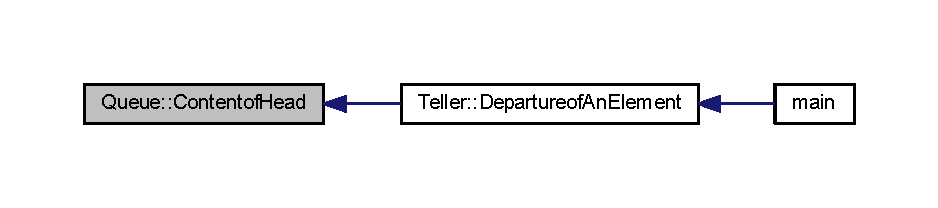
\includegraphics[width=350pt]{d4/da4/class_queue_ac3aa4048853f51c0552d532036b31cd6_icgraph}
\end{center}
\end{figure}


\hypertarget{class_queue_a019423c548927a8830677d1d2fddb38c}{\index{Queue@{Queue}!Contentof\-Tail@{Contentof\-Tail}}
\index{Contentof\-Tail@{Contentof\-Tail}!Queue@{Queue}}
\subsubsection[{Contentof\-Tail}]{\setlength{\rightskip}{0pt plus 5cm}int Queue\-::\-Contentof\-Tail (
\begin{DoxyParamCaption}
{}
\end{DoxyParamCaption}
)}}\label{class_queue_a019423c548927a8830677d1d2fddb38c}


Gets the content on \hyperlink{class_queue}{Queue}'s Tail address. 
\begin{DoxyExceptions}{Exceptions}
{\em Invalid\-Operation\-Exception} & \hyperlink{class_queue}{Queue} is empty. \\
\hline
\end{DoxyExceptions}


\begin{DoxyReturn}{Returns}
The value of \hyperlink{class_queue}{Queue}'s Tail address. 
\end{DoxyReturn}


Definition at line 93 of file Queue.\-cpp.

\hypertarget{class_queue_abee14281bbb50742493403315009822e}{\index{Queue@{Queue}!Deletefor\-Jockeying@{Deletefor\-Jockeying}}
\index{Deletefor\-Jockeying@{Deletefor\-Jockeying}!Queue@{Queue}}
\subsubsection[{Deletefor\-Jockeying}]{\setlength{\rightskip}{0pt plus 5cm}int Queue\-::\-Deletefor\-Jockeying (
\begin{DoxyParamCaption}
{}
\end{DoxyParamCaption}
)}}\label{class_queue_abee14281bbb50742493403315009822e}


Delete element on \hyperlink{class_queue}{Queue}'s Tail. 

\begin{DoxyReturn}{Returns}
Element on \hyperlink{class_queue}{Queue}'s Tail. 
\end{DoxyReturn}


Definition at line 169 of file Queue.\-cpp.



Here is the call graph for this function\-:\nopagebreak
\begin{figure}[H]
\begin{center}
\leavevmode
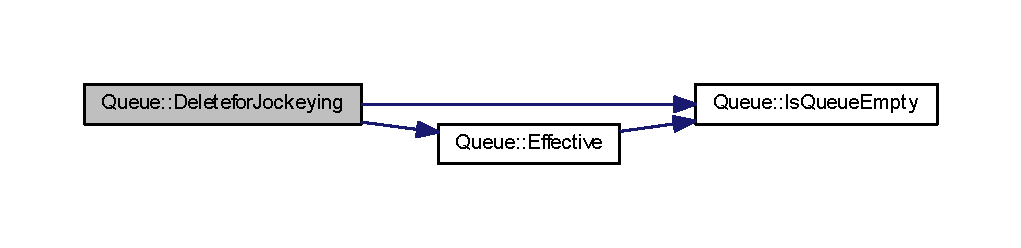
\includegraphics[width=350pt]{d4/da4/class_queue_abee14281bbb50742493403315009822e_cgraph}
\end{center}
\end{figure}




Here is the caller graph for this function\-:\nopagebreak
\begin{figure}[H]
\begin{center}
\leavevmode
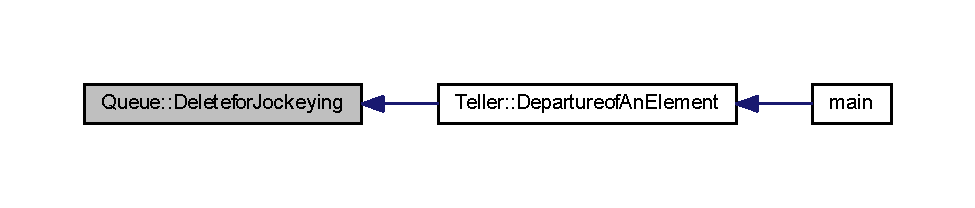
\includegraphics[width=350pt]{d4/da4/class_queue_abee14281bbb50742493403315009822e_icgraph}
\end{center}
\end{figure}


\hypertarget{class_queue_a298b3523c3f2ddda8dcc29c1aa499b26}{\index{Queue@{Queue}!Dequeue@{Dequeue}}
\index{Dequeue@{Dequeue}!Queue@{Queue}}
\subsubsection[{Dequeue}]{\setlength{\rightskip}{0pt plus 5cm}int Queue\-::\-Dequeue (
\begin{DoxyParamCaption}
{}
\end{DoxyParamCaption}
)}}\label{class_queue_a298b3523c3f2ddda8dcc29c1aa499b26}


Delete element on \hyperlink{class_queue}{Queue}'s Head. 

\begin{DoxyReturn}{Returns}
0 if \hyperlink{class_queue}{Queue} is empty; otherwise element on \hyperlink{class_queue}{Queue}'s Head. 
\end{DoxyReturn}


Definition at line 147 of file Queue.\-cpp.



Here is the call graph for this function\-:\nopagebreak
\begin{figure}[H]
\begin{center}
\leavevmode
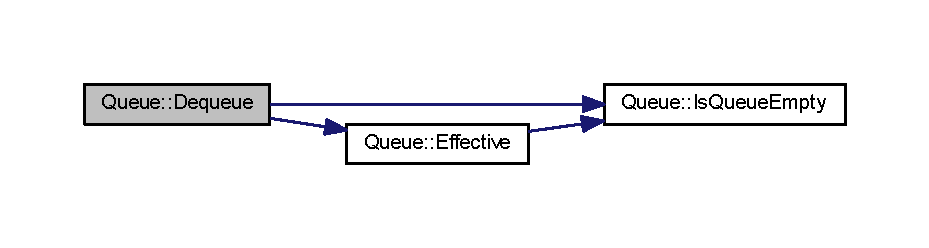
\includegraphics[width=350pt]{d4/da4/class_queue_a298b3523c3f2ddda8dcc29c1aa499b26_cgraph}
\end{center}
\end{figure}




Here is the caller graph for this function\-:\nopagebreak
\begin{figure}[H]
\begin{center}
\leavevmode
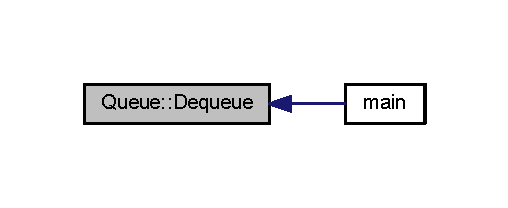
\includegraphics[width=244pt]{d4/da4/class_queue_a298b3523c3f2ddda8dcc29c1aa499b26_icgraph}
\end{center}
\end{figure}


\hypertarget{class_queue_ab9e0ba7176e94e7ee0ef75f0ef6120b0}{\index{Queue@{Queue}!Effective@{Effective}}
\index{Effective@{Effective}!Queue@{Queue}}
\subsubsection[{Effective}]{\setlength{\rightskip}{0pt plus 5cm}int Queue\-::\-Effective (
\begin{DoxyParamCaption}
{}
\end{DoxyParamCaption}
)}}\label{class_queue_ab9e0ba7176e94e7ee0ef75f0ef6120b0}


Gets the number of elements stored on \hyperlink{class_queue}{Queue}. 

\begin{DoxyReturn}{Returns}
The number of elements stored. 
\end{DoxyReturn}


Definition at line 111 of file Queue.\-cpp.



Here is the call graph for this function\-:\nopagebreak
\begin{figure}[H]
\begin{center}
\leavevmode
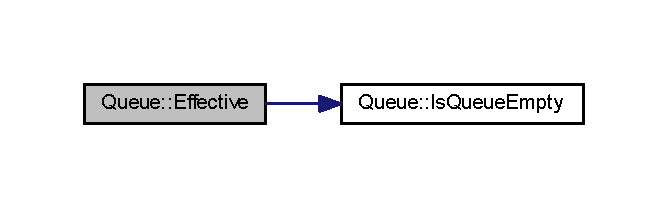
\includegraphics[width=320pt]{d4/da4/class_queue_ab9e0ba7176e94e7ee0ef75f0ef6120b0_cgraph}
\end{center}
\end{figure}




Here is the caller graph for this function\-:\nopagebreak
\begin{figure}[H]
\begin{center}
\leavevmode
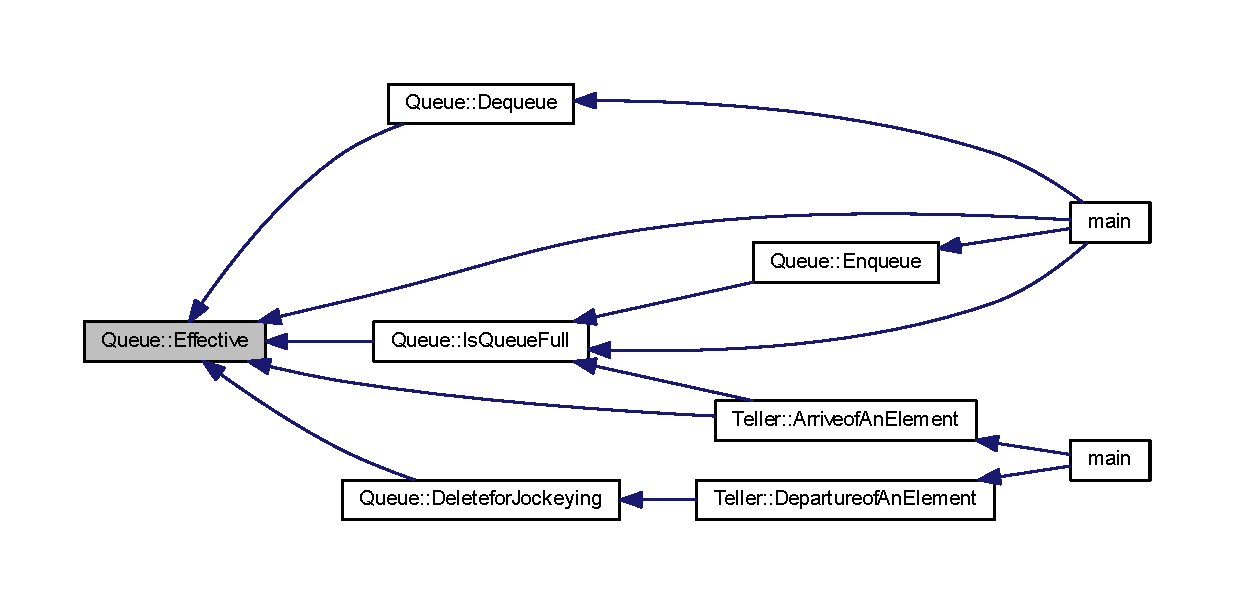
\includegraphics[width=350pt]{d4/da4/class_queue_ab9e0ba7176e94e7ee0ef75f0ef6120b0_icgraph}
\end{center}
\end{figure}


\hypertarget{class_queue_afe902699750ee1aa4600af72c4616957}{\index{Queue@{Queue}!Enqueue@{Enqueue}}
\index{Enqueue@{Enqueue}!Queue@{Queue}}
\subsubsection[{Enqueue}]{\setlength{\rightskip}{0pt plus 5cm}void Queue\-::\-Enqueue (
\begin{DoxyParamCaption}
\item[{int}]{Element}
\end{DoxyParamCaption}
)}}\label{class_queue_afe902699750ee1aa4600af72c4616957}


Add element to \hyperlink{class_queue}{Queue}'s Tail. 


\begin{DoxyParams}[1]{Parameters}
\mbox{\tt in}  & {\em Element} & Element to input. \\
\hline
\end{DoxyParams}


Definition at line 123 of file Queue.\-cpp.



Here is the call graph for this function\-:\nopagebreak
\begin{figure}[H]
\begin{center}
\leavevmode
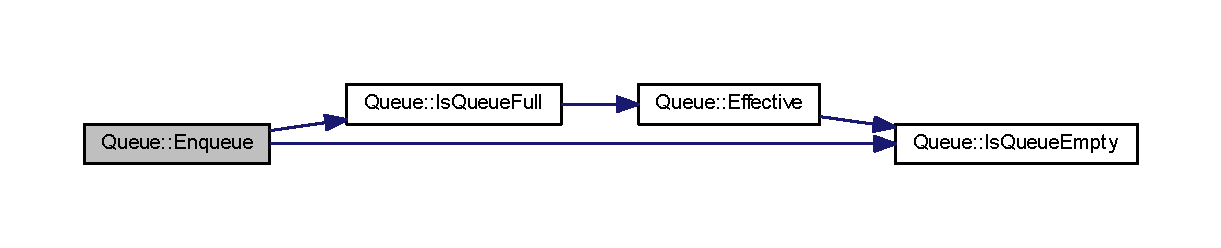
\includegraphics[width=350pt]{d4/da4/class_queue_afe902699750ee1aa4600af72c4616957_cgraph}
\end{center}
\end{figure}




Here is the caller graph for this function\-:\nopagebreak
\begin{figure}[H]
\begin{center}
\leavevmode
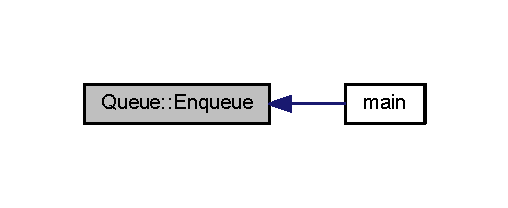
\includegraphics[width=244pt]{d4/da4/class_queue_afe902699750ee1aa4600af72c4616957_icgraph}
\end{center}
\end{figure}


\hypertarget{class_queue_abb997d38f5ac3bb506d8d073289affc1}{\index{Queue@{Queue}!Is\-Queue\-Empty@{Is\-Queue\-Empty}}
\index{Is\-Queue\-Empty@{Is\-Queue\-Empty}!Queue@{Queue}}
\subsubsection[{Is\-Queue\-Empty}]{\setlength{\rightskip}{0pt plus 5cm}bool Queue\-::\-Is\-Queue\-Empty (
\begin{DoxyParamCaption}
{}
\end{DoxyParamCaption}
)}}\label{class_queue_abb997d38f5ac3bb506d8d073289affc1}


Determines whether \hyperlink{class_queue}{Queue} is empty or not. 

\hyperlink{class_queue}{Queue} is empty if Head and Tail are 0. \begin{DoxyReturn}{Returns}
true if \hyperlink{class_queue}{Queue} is empty; otherwise false. 
\end{DoxyReturn}


Definition at line 101 of file Queue.\-cpp.



Here is the caller graph for this function\-:\nopagebreak
\begin{figure}[H]
\begin{center}
\leavevmode
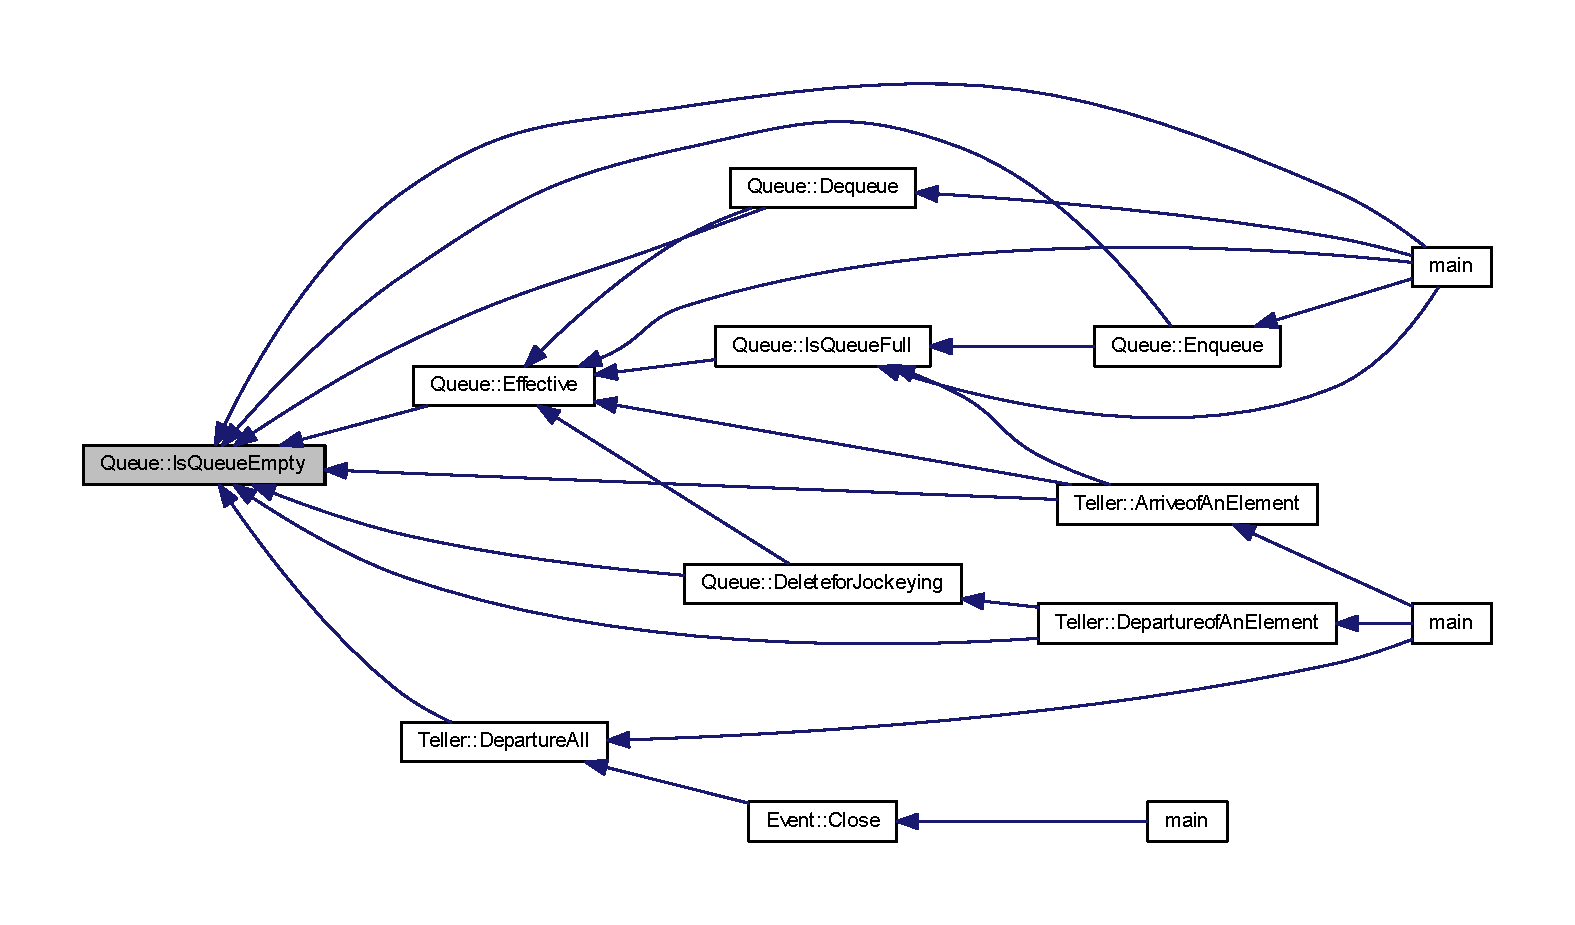
\includegraphics[width=350pt]{d4/da4/class_queue_abb997d38f5ac3bb506d8d073289affc1_icgraph}
\end{center}
\end{figure}


\hypertarget{class_queue_a2815639bf7c03ea9ccda9fa30c20f52e}{\index{Queue@{Queue}!Is\-Queue\-Full@{Is\-Queue\-Full}}
\index{Is\-Queue\-Full@{Is\-Queue\-Full}!Queue@{Queue}}
\subsubsection[{Is\-Queue\-Full}]{\setlength{\rightskip}{0pt plus 5cm}bool Queue\-::\-Is\-Queue\-Full (
\begin{DoxyParamCaption}
{}
\end{DoxyParamCaption}
)}}\label{class_queue_a2815639bf7c03ea9ccda9fa30c20f52e}


Determines whether \hyperlink{class_queue}{Queue} is full or not. 

\hyperlink{class_queue}{Queue} is full if Count() equals to the Maximum\-Capacityof\-Queue. \begin{DoxyReturn}{Returns}
true if \hyperlink{class_queue}{Queue} is full; otherwise false. 
\end{DoxyReturn}


Definition at line 106 of file Queue.\-cpp.



Here is the call graph for this function\-:\nopagebreak
\begin{figure}[H]
\begin{center}
\leavevmode
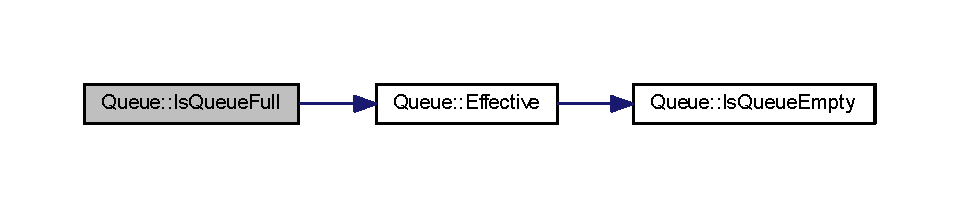
\includegraphics[width=350pt]{d4/da4/class_queue_a2815639bf7c03ea9ccda9fa30c20f52e_cgraph}
\end{center}
\end{figure}




Here is the caller graph for this function\-:\nopagebreak
\begin{figure}[H]
\begin{center}
\leavevmode
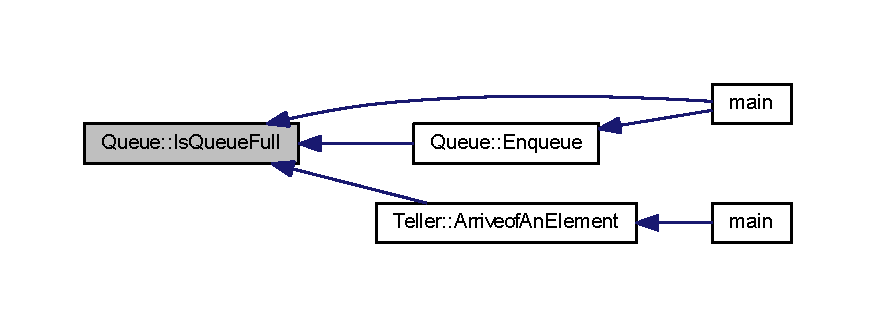
\includegraphics[width=350pt]{d4/da4/class_queue_a2815639bf7c03ea9ccda9fa30c20f52e_icgraph}
\end{center}
\end{figure}


\hypertarget{class_queue_a924ed23e355678aabd5d80551e9d3800}{\index{Queue@{Queue}!operator=@{operator=}}
\index{operator=@{operator=}!Queue@{Queue}}
\subsubsection[{operator=}]{\setlength{\rightskip}{0pt plus 5cm}{\bf Queue} \& Queue\-::operator= (
\begin{DoxyParamCaption}
\item[{const {\bf Queue} \&}]{Q}
\end{DoxyParamCaption}
)}}\label{class_queue_a924ed23e355678aabd5d80551e9d3800}


Copy all content of specified \hyperlink{class_queue}{Queue} to current \hyperlink{class_queue}{Queue}. 


\begin{DoxyParams}[1]{Parameters}
\mbox{\tt in}  & {\em Q} & The object \hyperlink{class_queue}{Queue} that will be copied. \\
\hline
\end{DoxyParams}


Definition at line 50 of file Queue.\-cpp.

\hypertarget{class_queue_a2b28fe3446577261546f74b7bbe3ccc6}{\index{Queue@{Queue}!Size@{Size}}
\index{Size@{Size}!Queue@{Queue}}
\subsubsection[{Size}]{\setlength{\rightskip}{0pt plus 5cm}int Queue\-::\-Size (
\begin{DoxyParamCaption}
{}
\end{DoxyParamCaption}
)}}\label{class_queue_a2b28fe3446577261546f74b7bbe3ccc6}


Gets the maximum capacity that can be stored on \hyperlink{class_queue}{Queue}. 

\begin{DoxyReturn}{Returns}
The maximum capacity of \hyperlink{class_queue}{Queue}. 
\end{DoxyReturn}


Definition at line 97 of file Queue.\-cpp.



Here is the caller graph for this function\-:\nopagebreak
\begin{figure}[H]
\begin{center}
\leavevmode
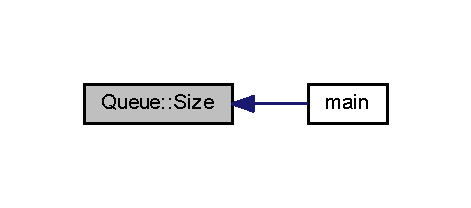
\includegraphics[width=226pt]{d4/da4/class_queue_a2b28fe3446577261546f74b7bbe3ccc6_icgraph}
\end{center}
\end{figure}




\subsection{Friends And Related Function Documentation}
\hypertarget{class_queue_aadecbaa986b78ce2a846e652d7bb57af}{\index{Queue@{Queue}!operator$<$$<$@{operator$<$$<$}}
\index{operator$<$$<$@{operator$<$$<$}!Queue@{Queue}}
\subsubsection[{operator$<$$<$}]{\setlength{\rightskip}{0pt plus 5cm}ostream\& operator$<$$<$ (
\begin{DoxyParamCaption}
\item[{ostream \&}]{output, }
\item[{const {\bf Queue} \&}]{Q}
\end{DoxyParamCaption}
)\hspace{0.3cm}{\ttfamily [friend]}}}\label{class_queue_aadecbaa986b78ce2a846e652d7bb57af}


Writes the specified \hyperlink{class_queue}{Queue} followed by the current line terminator to the standard output stream. 

\hyperlink{class_queue}{Queue} will be printed \{x1,x2,x3,...,xn\}


\begin{DoxyParams}[1]{Parameters}
\mbox{\tt out}  & {\em output} & An instance of class ostream. \\
\hline
\mbox{\tt in}  & {\em Q} & An instance of class \hyperlink{class_queue}{Queue}. \\
\hline
\end{DoxyParams}


Definition at line 69 of file Queue.\-h.



The documentation for this class was generated from the following files\-:\begin{DoxyCompactItemize}
\item 
Queue/\hyperlink{_queue_8h}{Queue.\-h}\item 
Queue/\hyperlink{_queue_8cpp}{Queue.\-cpp}\end{DoxyCompactItemize}

\hypertarget{class_teller}{\section{Teller Class Reference}
\label{class_teller}\index{Teller@{Teller}}
}


\hyperlink{class_teller}{Teller} Class.  




{\ttfamily \#include $<$Teller.\-h$>$}

\subsection*{Public Member Functions}
\begin{DoxyCompactItemize}
\item 
\hyperlink{class_teller_a652e56e65d8d73a53d709b8299e1c4a7}{Teller} ()
\begin{DoxyCompactList}\small\item\em Initializes a new instance of \hyperlink{class_teller}{Teller} class with 5 block \hyperlink{class_queue}{Queue}. \end{DoxyCompactList}\item 
\hyperlink{class_teller_a705ab8f9f4d16cba8f8ca9590d1598ca}{Teller} (int Numberof\-Teller)
\begin{DoxyCompactList}\small\item\em Initializes a new instance of \hyperlink{class_teller}{Teller} class with Numberof\-Teller block \hyperlink{class_queue}{Queue}. \end{DoxyCompactList}\item 
\hyperlink{class_teller_a96340cfc1acefbad9e329723dc08fabc}{Teller} (const \hyperlink{class_teller}{Teller} \&T)
\begin{DoxyCompactList}\small\item\em Initializes a new instance of the \hyperlink{class_teller}{Teller} class with all the content of specified \hyperlink{class_teller}{Teller}. \end{DoxyCompactList}\item 
\hyperlink{class_teller}{Teller} \& \hyperlink{class_teller_a8409f8ad1eb830534ad9d23d0ebacc57}{operator=} (const \hyperlink{class_teller}{Teller} \&T)
\begin{DoxyCompactList}\small\item\em Copy all content of specified \hyperlink{class_teller}{Teller} to current \hyperlink{class_teller}{Teller}. \end{DoxyCompactList}\item 
\hyperlink{class_teller_af61263c98d7ff236ca84ec551919d7e7}{$\sim$\-Teller} ()
\begin{DoxyCompactList}\small\item\em Clear an instance of \hyperlink{class_teller}{Teller} from memory. \end{DoxyCompactList}\item 
int \hyperlink{class_teller_a53829996d557a0bdf9513366461d7986}{Departureof\-An\-Element} (int I\-D)
\begin{DoxyCompactList}\small\item\em Delete element with the value I\-D from certain \hyperlink{class_queue}{Queue}. \end{DoxyCompactList}\item 
void \hyperlink{class_teller_ae5db2a5bde036fa0e0ff27f257cdea27}{Arriveof\-An\-Element} (int I\-D)
\begin{DoxyCompactList}\small\item\em Add element with the value I\-D to certain \hyperlink{class_queue}{Queue}. \end{DoxyCompactList}\item 
void \hyperlink{class_teller_a22b0dcc673d701ec82f88fa0cf58900a}{Departure\-All} ()
\begin{DoxyCompactList}\small\item\em Delete all element from all \hyperlink{class_queue}{Queue} and Print the element to console. \end{DoxyCompactList}\item 
void \hyperlink{class_teller_a85b5bfcdab1ad0f595f544bda26dea1e}{Print} ()
\begin{DoxyCompactList}\small\item\em Print all the \hyperlink{class_queue}{Queue} in \hyperlink{class_teller}{Teller}. \end{DoxyCompactList}\end{DoxyCompactItemize}


\subsection{Detailed Description}
\hyperlink{class_teller}{Teller} Class. 

Represent a \hyperlink{class_teller}{Teller}

\begin{DoxyAuthor}{Author}
Riva Syafri Rachmatullah (13512036) for .h file 

Riva Syafri Rachmatullah (13512036) for .cpp file
\end{DoxyAuthor}
\begin{DoxyVersion}{Version}
v1.\-3 
\end{DoxyVersion}


Definition at line 26 of file Teller.\-h.



\subsection{Constructor \& Destructor Documentation}
\hypertarget{class_teller_a652e56e65d8d73a53d709b8299e1c4a7}{\index{Teller@{Teller}!Teller@{Teller}}
\index{Teller@{Teller}!Teller@{Teller}}
\subsubsection[{Teller}]{\setlength{\rightskip}{0pt plus 5cm}Teller\-::\-Teller (
\begin{DoxyParamCaption}
{}
\end{DoxyParamCaption}
)}}\label{class_teller_a652e56e65d8d73a53d709b8299e1c4a7}


Initializes a new instance of \hyperlink{class_teller}{Teller} class with 5 block \hyperlink{class_queue}{Queue}. 



Definition at line 11 of file Teller.\-cpp.

\hypertarget{class_teller_a705ab8f9f4d16cba8f8ca9590d1598ca}{\index{Teller@{Teller}!Teller@{Teller}}
\index{Teller@{Teller}!Teller@{Teller}}
\subsubsection[{Teller}]{\setlength{\rightskip}{0pt plus 5cm}Teller\-::\-Teller (
\begin{DoxyParamCaption}
\item[{int}]{Numberof\-Teller}
\end{DoxyParamCaption}
)}}\label{class_teller_a705ab8f9f4d16cba8f8ca9590d1598ca}


Initializes a new instance of \hyperlink{class_teller}{Teller} class with Numberof\-Teller block \hyperlink{class_queue}{Queue}. 


\begin{DoxyParams}[1]{Parameters}
\mbox{\tt in}  & {\em Numberof\-Teller} & The number of teller. \\
\hline
\end{DoxyParams}


Definition at line 20 of file Teller.\-cpp.

\hypertarget{class_teller_a96340cfc1acefbad9e329723dc08fabc}{\index{Teller@{Teller}!Teller@{Teller}}
\index{Teller@{Teller}!Teller@{Teller}}
\subsubsection[{Teller}]{\setlength{\rightskip}{0pt plus 5cm}Teller\-::\-Teller (
\begin{DoxyParamCaption}
\item[{const {\bf Teller} \&}]{T}
\end{DoxyParamCaption}
)}}\label{class_teller_a96340cfc1acefbad9e329723dc08fabc}


Initializes a new instance of the \hyperlink{class_teller}{Teller} class with all the content of specified \hyperlink{class_teller}{Teller}. 


\begin{DoxyParams}[1]{Parameters}
\mbox{\tt in}  & {\em T} & The object \hyperlink{class_teller}{Teller} that will be copied. \\
\hline
\end{DoxyParams}


Definition at line 29 of file Teller.\-cpp.

\hypertarget{class_teller_af61263c98d7ff236ca84ec551919d7e7}{\index{Teller@{Teller}!$\sim$\-Teller@{$\sim$\-Teller}}
\index{$\sim$\-Teller@{$\sim$\-Teller}!Teller@{Teller}}
\subsubsection[{$\sim$\-Teller}]{\setlength{\rightskip}{0pt plus 5cm}Teller\-::$\sim$\-Teller (
\begin{DoxyParamCaption}
{}
\end{DoxyParamCaption}
)}}\label{class_teller_af61263c98d7ff236ca84ec551919d7e7}


Clear an instance of \hyperlink{class_teller}{Teller} from memory. 



Definition at line 59 of file Teller.\-cpp.



\subsection{Member Function Documentation}
\hypertarget{class_teller_ae5db2a5bde036fa0e0ff27f257cdea27}{\index{Teller@{Teller}!Arriveof\-An\-Element@{Arriveof\-An\-Element}}
\index{Arriveof\-An\-Element@{Arriveof\-An\-Element}!Teller@{Teller}}
\subsubsection[{Arriveof\-An\-Element}]{\setlength{\rightskip}{0pt plus 5cm}void Teller\-::\-Arriveof\-An\-Element (
\begin{DoxyParamCaption}
\item[{int}]{I\-D}
\end{DoxyParamCaption}
)}}\label{class_teller_ae5db2a5bde036fa0e0ff27f257cdea27}


Add element with the value I\-D to certain \hyperlink{class_queue}{Queue}. 

It will add element I\-D to the \hyperlink{class_queue}{Queue} who has the least number of element in \hyperlink{class_queue}{Queue}.


\begin{DoxyParams}[1]{Parameters}
\mbox{\tt in}  & {\em I\-D} & The element to add. \\
\hline
\end{DoxyParams}


Definition at line 93 of file Teller.\-cpp.



Here is the call graph for this function\-:\nopagebreak
\begin{figure}[H]
\begin{center}
\leavevmode
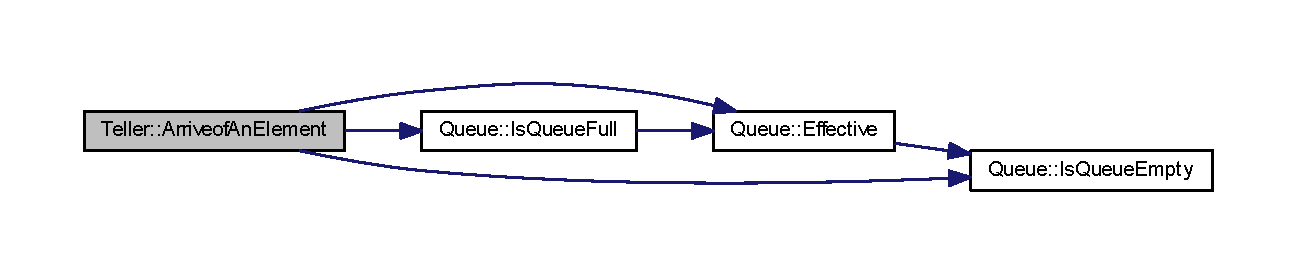
\includegraphics[width=350pt]{da/d18/class_teller_ae5db2a5bde036fa0e0ff27f257cdea27_cgraph}
\end{center}
\end{figure}




Here is the caller graph for this function\-:\nopagebreak
\begin{figure}[H]
\begin{center}
\leavevmode
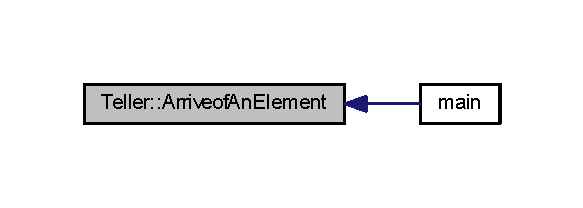
\includegraphics[width=280pt]{da/d18/class_teller_ae5db2a5bde036fa0e0ff27f257cdea27_icgraph}
\end{center}
\end{figure}


\hypertarget{class_teller_a22b0dcc673d701ec82f88fa0cf58900a}{\index{Teller@{Teller}!Departure\-All@{Departure\-All}}
\index{Departure\-All@{Departure\-All}!Teller@{Teller}}
\subsubsection[{Departure\-All}]{\setlength{\rightskip}{0pt plus 5cm}void Teller\-::\-Departure\-All (
\begin{DoxyParamCaption}
{}
\end{DoxyParamCaption}
)}}\label{class_teller_a22b0dcc673d701ec82f88fa0cf58900a}


Delete all element from all \hyperlink{class_queue}{Queue} and Print the element to console. 



Definition at line 109 of file Teller.\-cpp.



Here is the call graph for this function\-:\nopagebreak
\begin{figure}[H]
\begin{center}
\leavevmode
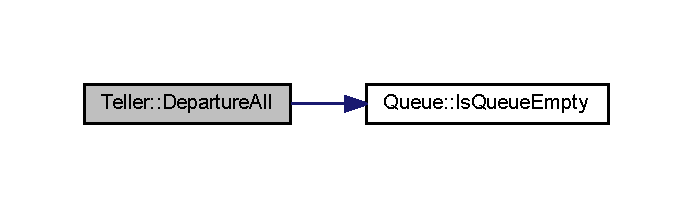
\includegraphics[width=332pt]{da/d18/class_teller_a22b0dcc673d701ec82f88fa0cf58900a_cgraph}
\end{center}
\end{figure}




Here is the caller graph for this function\-:\nopagebreak
\begin{figure}[H]
\begin{center}
\leavevmode
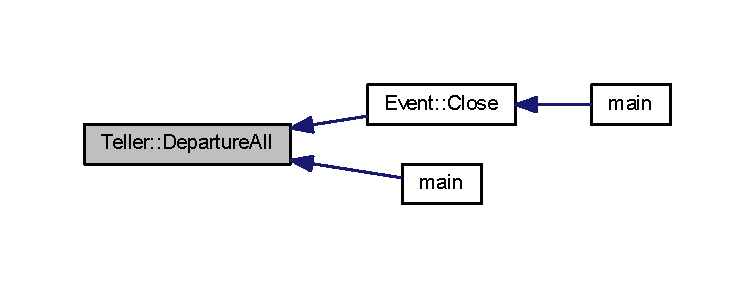
\includegraphics[width=350pt]{da/d18/class_teller_a22b0dcc673d701ec82f88fa0cf58900a_icgraph}
\end{center}
\end{figure}


\hypertarget{class_teller_a53829996d557a0bdf9513366461d7986}{\index{Teller@{Teller}!Departureof\-An\-Element@{Departureof\-An\-Element}}
\index{Departureof\-An\-Element@{Departureof\-An\-Element}!Teller@{Teller}}
\subsubsection[{Departureof\-An\-Element}]{\setlength{\rightskip}{0pt plus 5cm}int Teller\-::\-Departureof\-An\-Element (
\begin{DoxyParamCaption}
\item[{int}]{I\-D}
\end{DoxyParamCaption}
)}}\label{class_teller_a53829996d557a0bdf9513366461d7986}


Delete element with the value I\-D from certain \hyperlink{class_queue}{Queue}. 

This method does searching I\-D on \hyperlink{class_queue}{Queue}'s head address. If the I\-D isn't found then it will give a message and return 0.


\begin{DoxyParams}[1]{Parameters}
\mbox{\tt in}  & {\em I\-D} & The element to delete. \\
\hline
\end{DoxyParams}
\begin{DoxyReturn}{Returns}
I\-D of element if found; 0 if not found. 
\end{DoxyReturn}


Definition at line 65 of file Teller.\-cpp.



Here is the call graph for this function\-:\nopagebreak
\begin{figure}[H]
\begin{center}
\leavevmode
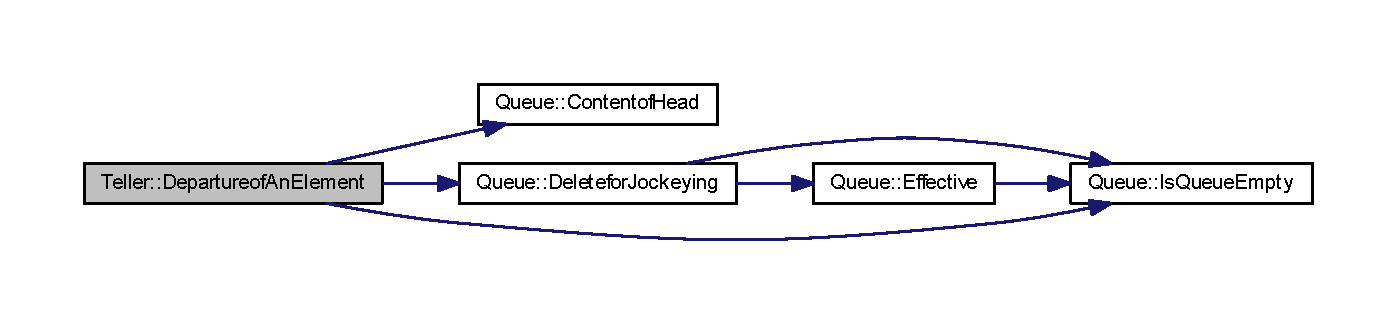
\includegraphics[width=350pt]{da/d18/class_teller_a53829996d557a0bdf9513366461d7986_cgraph}
\end{center}
\end{figure}




Here is the caller graph for this function\-:\nopagebreak
\begin{figure}[H]
\begin{center}
\leavevmode
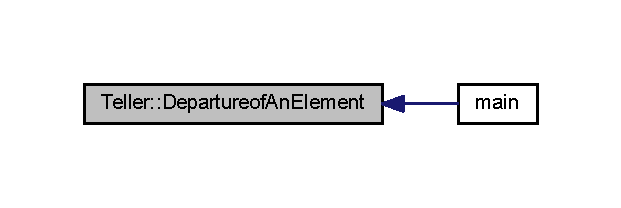
\includegraphics[width=298pt]{da/d18/class_teller_a53829996d557a0bdf9513366461d7986_icgraph}
\end{center}
\end{figure}


\hypertarget{class_teller_a8409f8ad1eb830534ad9d23d0ebacc57}{\index{Teller@{Teller}!operator=@{operator=}}
\index{operator=@{operator=}!Teller@{Teller}}
\subsubsection[{operator=}]{\setlength{\rightskip}{0pt plus 5cm}{\bf Teller} \& Teller\-::operator= (
\begin{DoxyParamCaption}
\item[{const {\bf Teller} \&}]{T}
\end{DoxyParamCaption}
)}}\label{class_teller_a8409f8ad1eb830534ad9d23d0ebacc57}


Copy all content of specified \hyperlink{class_teller}{Teller} to current \hyperlink{class_teller}{Teller}. 


\begin{DoxyParams}[1]{Parameters}
\mbox{\tt in}  & {\em T} & The object \hyperlink{class_teller}{Teller} that will be copied. \\
\hline
\end{DoxyParams}


Definition at line 41 of file Teller.\-cpp.

\hypertarget{class_teller_a85b5bfcdab1ad0f595f544bda26dea1e}{\index{Teller@{Teller}!Print@{Print}}
\index{Print@{Print}!Teller@{Teller}}
\subsubsection[{Print}]{\setlength{\rightskip}{0pt plus 5cm}void Teller\-::\-Print (
\begin{DoxyParamCaption}
{}
\end{DoxyParamCaption}
)}}\label{class_teller_a85b5bfcdab1ad0f595f544bda26dea1e}


Print all the \hyperlink{class_queue}{Queue} in \hyperlink{class_teller}{Teller}. 

Print will be printed like Qi = \{x1,x2,...,xn\} 

Definition at line 138 of file Teller.\-cpp.



Here is the caller graph for this function\-:\nopagebreak
\begin{figure}[H]
\begin{center}
\leavevmode
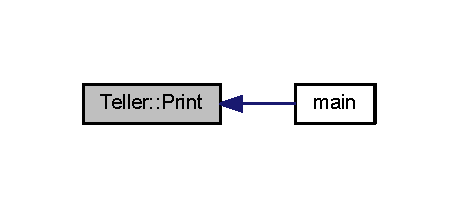
\includegraphics[width=220pt]{da/d18/class_teller_a85b5bfcdab1ad0f595f544bda26dea1e_icgraph}
\end{center}
\end{figure}




The documentation for this class was generated from the following files\-:\begin{DoxyCompactItemize}
\item 
Teller/\hyperlink{_teller_8h}{Teller.\-h}\item 
Teller/\hyperlink{_teller_8cpp}{Teller.\-cpp}\end{DoxyCompactItemize}

\hypertarget{class_time}{\section{Time Class Reference}
\label{class_time}\index{Time@{Time}}
}


\hyperlink{class_time}{Time} Class.  




{\ttfamily \#include $<$Time.\-h$>$}

\subsection*{Public Member Functions}
\begin{DoxyCompactItemize}
\item 
\hyperlink{class_time_a4245e409c7347d1d671858962c2ca3b5}{Time} ()
\begin{DoxyCompactList}\small\item\em Initializes a new instance of \hyperlink{class_time}{Time}. \end{DoxyCompactList}\item 
\hyperlink{class_time_aa90303dd0454141b15ceb358d60795a4}{Time} (const \hyperlink{class_time}{Time} \&T)
\begin{DoxyCompactList}\small\item\em Initializes a new instance of \hyperlink{class_time}{Time} from specified \hyperlink{class_time}{Time} instance. \end{DoxyCompactList}\item 
\hyperlink{class_time_a1e92dbe963fa3cdd6bea207680f5f6d1}{$\sim$\-Time} ()
\begin{DoxyCompactList}\small\item\em Clear an instance of \hyperlink{class_time}{Time} from memory. \end{DoxyCompactList}\item 
bool \hyperlink{class_time_a0e5c32707d684d728e2b2f4f33748cf0}{operator==} (const \hyperlink{class_time}{Time} \&T)
\begin{DoxyCompactList}\small\item\em Determines whether the specified object \hyperlink{class_time}{Time} is equal to the current object \hyperlink{class_time}{Time}. \end{DoxyCompactList}\item 
bool \hyperlink{class_time_aa582792aedd7600a67245f574650dcb5}{operator!=} (const \hyperlink{class_time}{Time} \&T)
\begin{DoxyCompactList}\small\item\em Determines whether the specified object \hyperlink{class_time}{Time} is not equal to the current object \hyperlink{class_time}{Time}. \end{DoxyCompactList}\item 
bool \hyperlink{class_time_a2105a3d96442b30c78de1c39cfe78a43}{operator$<$} (const \hyperlink{class_time}{Time} \&T)
\begin{DoxyCompactList}\small\item\em Determines whether the specified object \hyperlink{class_time}{Time} is earlier than the current object \hyperlink{class_time}{Time}. \end{DoxyCompactList}\item 
bool \hyperlink{class_time_a5685f6f63cfad7d5e87aaac121bdc455}{operator$>$} (const \hyperlink{class_time}{Time} \&T)
\begin{DoxyCompactList}\small\item\em Determines whether the specified object \hyperlink{class_time}{Time} is later than the current object \hyperlink{class_time}{Time}. \end{DoxyCompactList}\item 
int \hyperlink{class_time_a48e43f8a54d938d4ffbf6443c73b4ffd}{Get\-Hour\-Element} ()
\begin{DoxyCompactList}\small\item\em Gets the hour element of specified \hyperlink{class_time}{Time}. \end{DoxyCompactList}\item 
int \hyperlink{class_time_a1aa88252331ef2e9f91a3ffe82e3d378}{Get\-Minute\-Element} ()
\begin{DoxyCompactList}\small\item\em Gets the minute element of specified \hyperlink{class_time}{Time}. \end{DoxyCompactList}\item 
int \hyperlink{class_time_a998ba1fdc211afdc48bae6b74412f609}{Get\-Second\-Element} ()
\begin{DoxyCompactList}\small\item\em Gets the second element of specified \hyperlink{class_time}{Time}. \end{DoxyCompactList}\item 
void \hyperlink{class_time_a97e5d72787a0b47c786349df031b44e8}{Set\-Hour\-Element} (int Hour\-Element)
\begin{DoxyCompactList}\small\item\em Set the hour element of time with specified hour. \end{DoxyCompactList}\item 
void \hyperlink{class_time_a5cbba1ef9416cc8466b60e2ef789bd86}{Set\-Minute\-Element} (int Minute\-Element)
\begin{DoxyCompactList}\small\item\em Set the minute element of time with specified minute. \end{DoxyCompactList}\item 
void \hyperlink{class_time_ad100ad8e6e9bc35043881c697f7efef1}{Set\-Second\-Element} (int Second\-Element)
\begin{DoxyCompactList}\small\item\em Set the second element of time with specified second. \end{DoxyCompactList}\end{DoxyCompactItemize}
\subsection*{Static Public Member Functions}
\begin{DoxyCompactItemize}
\item 
static bool \hyperlink{class_time_a73518dd61e22a29dded0c808a746e6be}{Is\-Elementof\-Time\-Valid} (int Hour\-Element, int Minute\-Element, int Second\-Element)
\begin{DoxyCompactList}\small\item\em Determines if the specified elements of time is a valid time. \end{DoxyCompactList}\end{DoxyCompactItemize}
\subsection*{Friends}
\begin{DoxyCompactItemize}
\item 
ostream \& \hyperlink{class_time_af7462b6d18ba08745290b681487bed88}{operator$<$$<$} (ostream \&output, const \hyperlink{class_time}{Time} \&T)
\begin{DoxyCompactList}\small\item\em Writes the specified \hyperlink{class_time}{Time} followed by the current line terminator to the standard output stream. \end{DoxyCompactList}\item 
istream \& \hyperlink{class_time_af8dde22bf0e747b2b3525ff7b8d648f4}{operator$>$$>$} (istream \&input, \hyperlink{class_time}{Time} \&T)
\begin{DoxyCompactList}\small\item\em Read the specified \hyperlink{class_time}{Time} to the standard input stream. \end{DoxyCompactList}\end{DoxyCompactItemize}


\subsection{Detailed Description}
\hyperlink{class_time}{Time} Class. 

Represent a \hyperlink{class_time}{Time}

\begin{DoxyAuthor}{Author}
Riva Syafri Rachmatullah (13512036) for .h file 

Indam Muhammad (13512026) and Riva Syafri Rachmatullah (13512036) for .cpp file
\end{DoxyAuthor}
\begin{DoxyVersion}{Version}
v1.\-2 
\end{DoxyVersion}


Definition at line 25 of file Time.\-h.



\subsection{Constructor \& Destructor Documentation}
\hypertarget{class_time_a4245e409c7347d1d671858962c2ca3b5}{\index{Time@{Time}!Time@{Time}}
\index{Time@{Time}!Time@{Time}}
\subsubsection[{Time}]{\setlength{\rightskip}{0pt plus 5cm}Time\-::\-Time (
\begin{DoxyParamCaption}
{}
\end{DoxyParamCaption}
)}}\label{class_time_a4245e409c7347d1d671858962c2ca3b5}


Initializes a new instance of \hyperlink{class_time}{Time}. 



Definition at line 8 of file Time.\-cpp.

\hypertarget{class_time_aa90303dd0454141b15ceb358d60795a4}{\index{Time@{Time}!Time@{Time}}
\index{Time@{Time}!Time@{Time}}
\subsubsection[{Time}]{\setlength{\rightskip}{0pt plus 5cm}Time\-::\-Time (
\begin{DoxyParamCaption}
\item[{const {\bf Time} \&}]{T}
\end{DoxyParamCaption}
)}}\label{class_time_aa90303dd0454141b15ceb358d60795a4}


Initializes a new instance of \hyperlink{class_time}{Time} from specified \hyperlink{class_time}{Time} instance. 


\begin{DoxyParams}[1]{Parameters}
\mbox{\tt in}  & {\em T} & The object \hyperlink{class_time}{Time} that will be copied. \\
\hline
\end{DoxyParams}


Definition at line 15 of file Time.\-cpp.

\hypertarget{class_time_a1e92dbe963fa3cdd6bea207680f5f6d1}{\index{Time@{Time}!$\sim$\-Time@{$\sim$\-Time}}
\index{$\sim$\-Time@{$\sim$\-Time}!Time@{Time}}
\subsubsection[{$\sim$\-Time}]{\setlength{\rightskip}{0pt plus 5cm}Time\-::$\sim$\-Time (
\begin{DoxyParamCaption}
{}
\end{DoxyParamCaption}
)}}\label{class_time_a1e92dbe963fa3cdd6bea207680f5f6d1}


Clear an instance of \hyperlink{class_time}{Time} from memory. 



Definition at line 22 of file Time.\-cpp.



\subsection{Member Function Documentation}
\hypertarget{class_time_a48e43f8a54d938d4ffbf6443c73b4ffd}{\index{Time@{Time}!Get\-Hour\-Element@{Get\-Hour\-Element}}
\index{Get\-Hour\-Element@{Get\-Hour\-Element}!Time@{Time}}
\subsubsection[{Get\-Hour\-Element}]{\setlength{\rightskip}{0pt plus 5cm}int Time\-::\-Get\-Hour\-Element (
\begin{DoxyParamCaption}
{}
\end{DoxyParamCaption}
)}}\label{class_time_a48e43f8a54d938d4ffbf6443c73b4ffd}


Gets the hour element of specified \hyperlink{class_time}{Time}. 

\begin{DoxyReturn}{Returns}
The hour element of time. 
\end{DoxyReturn}


Definition at line 71 of file Time.\-cpp.

\hypertarget{class_time_a1aa88252331ef2e9f91a3ffe82e3d378}{\index{Time@{Time}!Get\-Minute\-Element@{Get\-Minute\-Element}}
\index{Get\-Minute\-Element@{Get\-Minute\-Element}!Time@{Time}}
\subsubsection[{Get\-Minute\-Element}]{\setlength{\rightskip}{0pt plus 5cm}int Time\-::\-Get\-Minute\-Element (
\begin{DoxyParamCaption}
{}
\end{DoxyParamCaption}
)}}\label{class_time_a1aa88252331ef2e9f91a3ffe82e3d378}


Gets the minute element of specified \hyperlink{class_time}{Time}. 

\begin{DoxyReturn}{Returns}
The minute element of time. 
\end{DoxyReturn}


Definition at line 75 of file Time.\-cpp.

\hypertarget{class_time_a998ba1fdc211afdc48bae6b74412f609}{\index{Time@{Time}!Get\-Second\-Element@{Get\-Second\-Element}}
\index{Get\-Second\-Element@{Get\-Second\-Element}!Time@{Time}}
\subsubsection[{Get\-Second\-Element}]{\setlength{\rightskip}{0pt plus 5cm}int Time\-::\-Get\-Second\-Element (
\begin{DoxyParamCaption}
{}
\end{DoxyParamCaption}
)}}\label{class_time_a998ba1fdc211afdc48bae6b74412f609}


Gets the second element of specified \hyperlink{class_time}{Time}. 

\begin{DoxyReturn}{Returns}
The second element of time. 
\end{DoxyReturn}


Definition at line 79 of file Time.\-cpp.

\hypertarget{class_time_a73518dd61e22a29dded0c808a746e6be}{\index{Time@{Time}!Is\-Elementof\-Time\-Valid@{Is\-Elementof\-Time\-Valid}}
\index{Is\-Elementof\-Time\-Valid@{Is\-Elementof\-Time\-Valid}!Time@{Time}}
\subsubsection[{Is\-Elementof\-Time\-Valid}]{\setlength{\rightskip}{0pt plus 5cm}bool Time\-::\-Is\-Elementof\-Time\-Valid (
\begin{DoxyParamCaption}
\item[{int}]{Hour\-Element, }
\item[{int}]{Minute\-Element, }
\item[{int}]{Second\-Element}
\end{DoxyParamCaption}
)\hspace{0.3cm}{\ttfamily [static]}}}\label{class_time_a73518dd61e22a29dded0c808a746e6be}


Determines if the specified elements of time is a valid time. 

Elements of \hyperlink{class_time}{Time} will be valid if Hour\-Element is equal and between 0 to 23 with Minute\-Element and Second\-Element are equal and between 0 to 59.


\begin{DoxyParams}[1]{Parameters}
\mbox{\tt in}  & {\em Hour\-Element} & The hour element of time. \\
\hline
\mbox{\tt in}  & {\em Minute\-Element} & The minute element of time. \\
\hline
\mbox{\tt in}  & {\em Second\-Element} & The second element of time. \\
\hline
\end{DoxyParams}
\begin{DoxyReturn}{Returns}
true if all elements of \hyperlink{class_time}{Time} is valid. 
\end{DoxyReturn}


Definition at line 64 of file Time.\-cpp.



Here is the caller graph for this function\-:\nopagebreak
\begin{figure}[H]
\begin{center}
\leavevmode
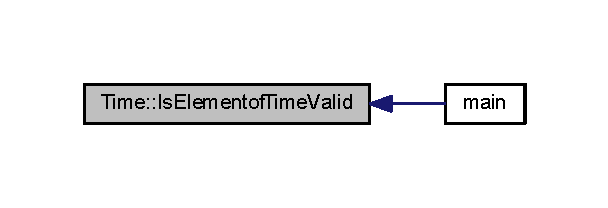
\includegraphics[width=292pt]{d6/d2c/class_time_a73518dd61e22a29dded0c808a746e6be_icgraph}
\end{center}
\end{figure}


\hypertarget{class_time_aa582792aedd7600a67245f574650dcb5}{\index{Time@{Time}!operator!=@{operator!=}}
\index{operator!=@{operator!=}!Time@{Time}}
\subsubsection[{operator!=}]{\setlength{\rightskip}{0pt plus 5cm}bool Time\-::operator!= (
\begin{DoxyParamCaption}
\item[{const {\bf Time} \&}]{T}
\end{DoxyParamCaption}
)}}\label{class_time_aa582792aedd7600a67245f574650dcb5}


Determines whether the specified object \hyperlink{class_time}{Time} is not equal to the current object \hyperlink{class_time}{Time}. 


\begin{DoxyParams}[1]{Parameters}
\mbox{\tt in}  & {\em T} & The object \hyperlink{class_time}{Time} to compare with the current object \hyperlink{class_time}{Time}. \\
\hline
\end{DoxyParams}
\begin{DoxyReturn}{Returns}
true if the specified object \hyperlink{class_time}{Time} is not equal to the current object \hyperlink{class_time}{Time}; otherwise false. 
\end{DoxyReturn}


Definition at line 31 of file Time.\-cpp.

\hypertarget{class_time_a2105a3d96442b30c78de1c39cfe78a43}{\index{Time@{Time}!operator$<$@{operator$<$}}
\index{operator$<$@{operator$<$}!Time@{Time}}
\subsubsection[{operator$<$}]{\setlength{\rightskip}{0pt plus 5cm}bool Time\-::operator$<$ (
\begin{DoxyParamCaption}
\item[{const {\bf Time} \&}]{T}
\end{DoxyParamCaption}
)}}\label{class_time_a2105a3d96442b30c78de1c39cfe78a43}


Determines whether the specified object \hyperlink{class_time}{Time} is earlier than the current object \hyperlink{class_time}{Time}. 


\begin{DoxyParams}[1]{Parameters}
\mbox{\tt in}  & {\em T} & The object \hyperlink{class_time}{Time} to compare with the current object \hyperlink{class_time}{Time}. \\
\hline
\end{DoxyParams}
\begin{DoxyReturn}{Returns}
true if the specified object \hyperlink{class_time}{Time} is earlier than the current object \hyperlink{class_time}{Time}; otherwise false. 
\end{DoxyReturn}


Definition at line 38 of file Time.\-cpp.

\hypertarget{class_time_a0e5c32707d684d728e2b2f4f33748cf0}{\index{Time@{Time}!operator==@{operator==}}
\index{operator==@{operator==}!Time@{Time}}
\subsubsection[{operator==}]{\setlength{\rightskip}{0pt plus 5cm}bool Time\-::operator== (
\begin{DoxyParamCaption}
\item[{const {\bf Time} \&}]{T}
\end{DoxyParamCaption}
)}}\label{class_time_a0e5c32707d684d728e2b2f4f33748cf0}


Determines whether the specified object \hyperlink{class_time}{Time} is equal to the current object \hyperlink{class_time}{Time}. 


\begin{DoxyParams}[1]{Parameters}
\mbox{\tt in}  & {\em T} & The object \hyperlink{class_time}{Time} to compare with the current object \hyperlink{class_time}{Time}. \\
\hline
\end{DoxyParams}
\begin{DoxyReturn}{Returns}
true if the specified object \hyperlink{class_time}{Time} is equal to the current object \hyperlink{class_time}{Time}; otherwise false. 
\end{DoxyReturn}


Definition at line 24 of file Time.\-cpp.

\hypertarget{class_time_a5685f6f63cfad7d5e87aaac121bdc455}{\index{Time@{Time}!operator$>$@{operator$>$}}
\index{operator$>$@{operator$>$}!Time@{Time}}
\subsubsection[{operator$>$}]{\setlength{\rightskip}{0pt plus 5cm}bool Time\-::operator$>$ (
\begin{DoxyParamCaption}
\item[{const {\bf Time} \&}]{T}
\end{DoxyParamCaption}
)}}\label{class_time_a5685f6f63cfad7d5e87aaac121bdc455}


Determines whether the specified object \hyperlink{class_time}{Time} is later than the current object \hyperlink{class_time}{Time}. 


\begin{DoxyParams}[1]{Parameters}
\mbox{\tt in}  & {\em T} & The object \hyperlink{class_time}{Time} to compare with the current object \hyperlink{class_time}{Time}. \\
\hline
\end{DoxyParams}
\begin{DoxyReturn}{Returns}
true if the specified object \hyperlink{class_time}{Time} is later than the current object \hyperlink{class_time}{Time}; otherwise false. 
\end{DoxyReturn}


Definition at line 51 of file Time.\-cpp.

\hypertarget{class_time_a97e5d72787a0b47c786349df031b44e8}{\index{Time@{Time}!Set\-Hour\-Element@{Set\-Hour\-Element}}
\index{Set\-Hour\-Element@{Set\-Hour\-Element}!Time@{Time}}
\subsubsection[{Set\-Hour\-Element}]{\setlength{\rightskip}{0pt plus 5cm}void Time\-::\-Set\-Hour\-Element (
\begin{DoxyParamCaption}
\item[{int}]{Hour\-Element}
\end{DoxyParamCaption}
)}}\label{class_time_a97e5d72787a0b47c786349df031b44e8}


Set the hour element of time with specified hour. 

Parameter must be a valid Hour\-Element.


\begin{DoxyParams}[1]{Parameters}
\mbox{\tt in}  & {\em Hour\-Element} & The new hour element of time. \\
\hline
\end{DoxyParams}


Definition at line 83 of file Time.\-cpp.



Here is the caller graph for this function\-:\nopagebreak
\begin{figure}[H]
\begin{center}
\leavevmode
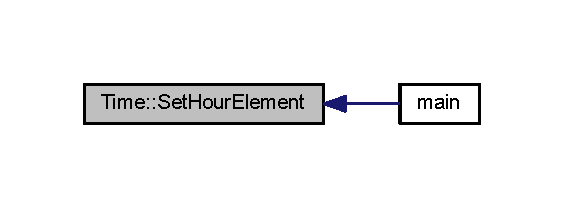
\includegraphics[width=270pt]{d6/d2c/class_time_a97e5d72787a0b47c786349df031b44e8_icgraph}
\end{center}
\end{figure}


\hypertarget{class_time_a5cbba1ef9416cc8466b60e2ef789bd86}{\index{Time@{Time}!Set\-Minute\-Element@{Set\-Minute\-Element}}
\index{Set\-Minute\-Element@{Set\-Minute\-Element}!Time@{Time}}
\subsubsection[{Set\-Minute\-Element}]{\setlength{\rightskip}{0pt plus 5cm}void Time\-::\-Set\-Minute\-Element (
\begin{DoxyParamCaption}
\item[{int}]{Minute\-Element}
\end{DoxyParamCaption}
)}}\label{class_time_a5cbba1ef9416cc8466b60e2ef789bd86}


Set the minute element of time with specified minute. 

Parameter must be a valid Minute\-Element.


\begin{DoxyParams}[1]{Parameters}
\mbox{\tt in}  & {\em Minute\-Element} & The new minute element of time. \\
\hline
\end{DoxyParams}


Definition at line 87 of file Time.\-cpp.



Here is the caller graph for this function\-:\nopagebreak
\begin{figure}[H]
\begin{center}
\leavevmode
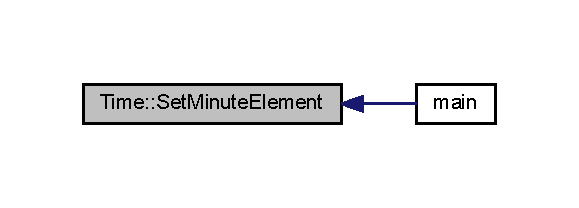
\includegraphics[width=278pt]{d6/d2c/class_time_a5cbba1ef9416cc8466b60e2ef789bd86_icgraph}
\end{center}
\end{figure}


\hypertarget{class_time_ad100ad8e6e9bc35043881c697f7efef1}{\index{Time@{Time}!Set\-Second\-Element@{Set\-Second\-Element}}
\index{Set\-Second\-Element@{Set\-Second\-Element}!Time@{Time}}
\subsubsection[{Set\-Second\-Element}]{\setlength{\rightskip}{0pt plus 5cm}void Time\-::\-Set\-Second\-Element (
\begin{DoxyParamCaption}
\item[{int}]{Second\-Element}
\end{DoxyParamCaption}
)}}\label{class_time_ad100ad8e6e9bc35043881c697f7efef1}


Set the second element of time with specified second. 

Parameter must be a valid Second\-Element.


\begin{DoxyParams}[1]{Parameters}
\mbox{\tt in}  & {\em Second\-Element} & The new second element of time. \\
\hline
\end{DoxyParams}


Definition at line 91 of file Time.\-cpp.



Here is the caller graph for this function\-:\nopagebreak
\begin{figure}[H]
\begin{center}
\leavevmode
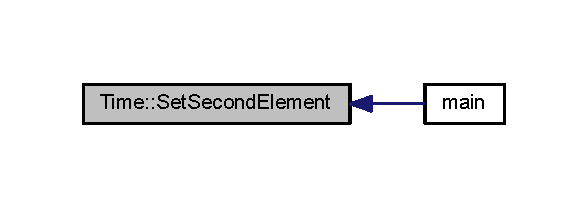
\includegraphics[width=282pt]{d6/d2c/class_time_ad100ad8e6e9bc35043881c697f7efef1_icgraph}
\end{center}
\end{figure}




\subsection{Friends And Related Function Documentation}
\hypertarget{class_time_af7462b6d18ba08745290b681487bed88}{\index{Time@{Time}!operator$<$$<$@{operator$<$$<$}}
\index{operator$<$$<$@{operator$<$$<$}!Time@{Time}}
\subsubsection[{operator$<$$<$}]{\setlength{\rightskip}{0pt plus 5cm}ostream\& operator$<$$<$ (
\begin{DoxyParamCaption}
\item[{ostream \&}]{output, }
\item[{const {\bf Time} \&}]{T}
\end{DoxyParamCaption}
)\hspace{0.3cm}{\ttfamily [friend]}}}\label{class_time_af7462b6d18ba08745290b681487bed88}


Writes the specified \hyperlink{class_time}{Time} followed by the current line terminator to the standard output stream. 


\begin{DoxyParams}[1]{Parameters}
\mbox{\tt out}  & {\em output} & An instance of class ostream. \\
\hline
\mbox{\tt in}  & {\em T} & An instance of class \hyperlink{class_time}{Time}. \\
\hline
\end{DoxyParams}


Definition at line 86 of file Time.\-h.

\hypertarget{class_time_af8dde22bf0e747b2b3525ff7b8d648f4}{\index{Time@{Time}!operator$>$$>$@{operator$>$$>$}}
\index{operator$>$$>$@{operator$>$$>$}!Time@{Time}}
\subsubsection[{operator$>$$>$}]{\setlength{\rightskip}{0pt plus 5cm}istream\& operator$>$$>$ (
\begin{DoxyParamCaption}
\item[{istream \&}]{input, }
\item[{{\bf Time} \&}]{T}
\end{DoxyParamCaption}
)\hspace{0.3cm}{\ttfamily [friend]}}}\label{class_time_af8dde22bf0e747b2b3525ff7b8d648f4}


Read the specified \hyperlink{class_time}{Time} to the standard input stream. 


\begin{DoxyParams}[1]{Parameters}
\mbox{\tt out}  & {\em input} & An instance of class istream. \\
\hline
\mbox{\tt out}  & {\em T} & An instance of class \hyperlink{class_time}{Time}. \\
\hline
\end{DoxyParams}


Definition at line 98 of file Time.\-h.



The documentation for this class was generated from the following files\-:\begin{DoxyCompactItemize}
\item 
Time/\hyperlink{_time_8h}{Time.\-h}\item 
Time/\hyperlink{_time_8cpp}{Time.\-cpp}\end{DoxyCompactItemize}

\chapter{File Documentation}
\hypertarget{_date_8cpp}{\section{Date/\-Date.cpp File Reference}
\label{_date_8cpp}\index{Date/\-Date.\-cpp@{Date/\-Date.\-cpp}}
}


Implementation \hyperlink{class_date}{Date} Class.  


{\ttfamily \#include \char`\"{}Date.\-h\char`\"{}}\\*
Include dependency graph for Date.\-cpp\-:\nopagebreak
\begin{figure}[H]
\begin{center}
\leavevmode
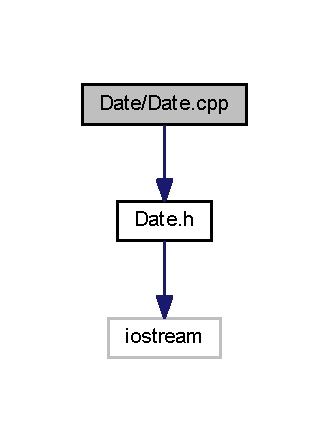
\includegraphics[width=158pt]{df/d5c/_date_8cpp__incl}
\end{center}
\end{figure}


\subsection{Detailed Description}
Implementation \hyperlink{class_date}{Date} Class. 

Definition in file \hyperlink{_date_8cpp_source}{Date.\-cpp}.


\hypertarget{_date_8h}{\section{Date/\-Date.h File Reference}
\label{_date_8h}\index{Date/\-Date.\-h@{Date/\-Date.\-h}}
}


Header \hyperlink{class_date}{Date} Class.  


{\ttfamily \#include $<$iostream$>$}\\*
Include dependency graph for Date.\-h\-:\nopagebreak
\begin{figure}[H]
\begin{center}
\leavevmode
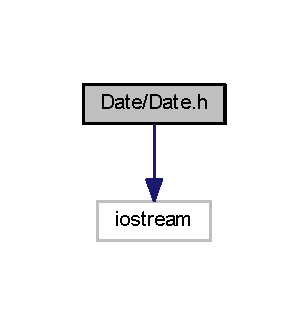
\includegraphics[width=148pt]{db/deb/_date_8h__incl}
\end{center}
\end{figure}
This graph shows which files directly or indirectly include this file\-:\nopagebreak
\begin{figure}[H]
\begin{center}
\leavevmode
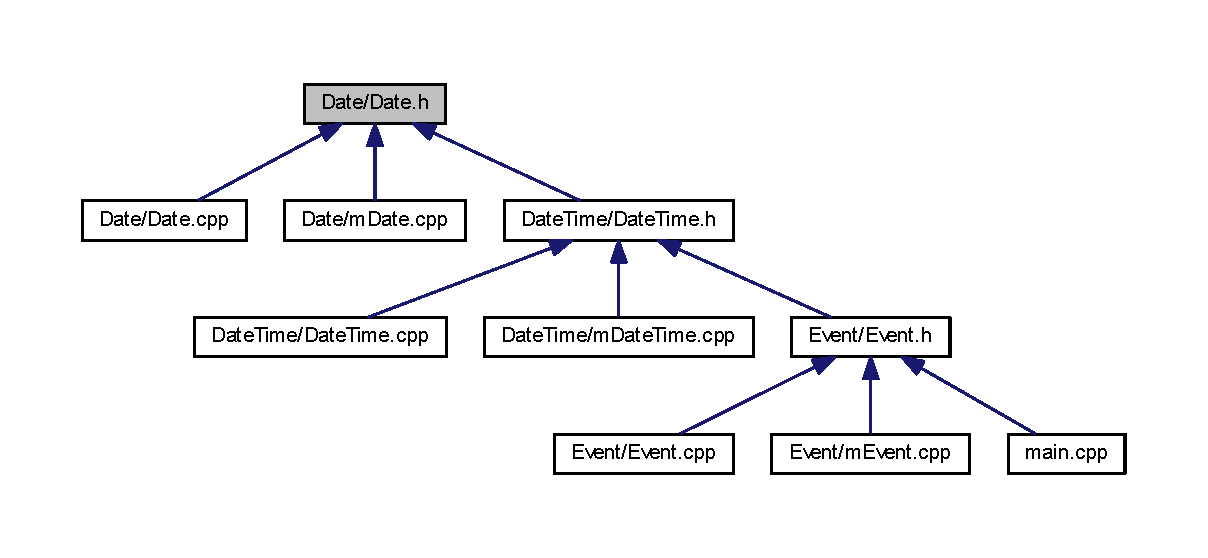
\includegraphics[width=350pt]{d8/d4d/_date_8h__dep__incl}
\end{center}
\end{figure}
\subsection*{Classes}
\begin{DoxyCompactItemize}
\item 
class \hyperlink{class_date}{Date}
\begin{DoxyCompactList}\small\item\em \hyperlink{class_date}{Date} Class. \end{DoxyCompactList}\end{DoxyCompactItemize}


\subsection{Detailed Description}
Header \hyperlink{class_date}{Date} Class. 

Definition in file \hyperlink{_date_8h_source}{Date.\-h}.


\hypertarget{m_date_8cpp}{\section{Date/m\-Date.cpp File Reference}
\label{m_date_8cpp}\index{Date/m\-Date.\-cpp@{Date/m\-Date.\-cpp}}
}


Driver \hyperlink{class_date}{Date} Class.  


{\ttfamily \#include $<$iostream$>$}\\*
{\ttfamily \#include \char`\"{}Date.\-h\char`\"{}}\\*
Include dependency graph for m\-Date.\-cpp\-:\nopagebreak
\begin{figure}[H]
\begin{center}
\leavevmode
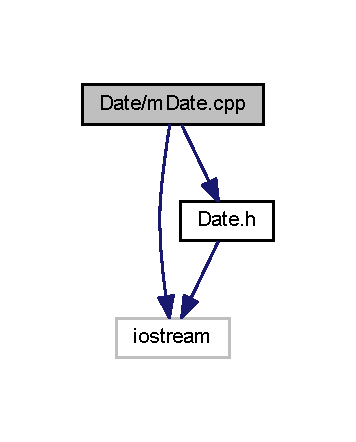
\includegraphics[width=171pt]{d6/d83/m_date_8cpp__incl}
\end{center}
\end{figure}
\subsection*{Functions}
\begin{DoxyCompactItemize}
\item 
void \hyperlink{m_date_8cpp_afdf1ca9e7afc3e7ec41b47fea4b3d80d}{Menu} ()
\item 
int \hyperlink{m_date_8cpp_ae66f6b31b5ad750f1fe042a706a4e3d4}{main} ()
\end{DoxyCompactItemize}


\subsection{Detailed Description}
Driver \hyperlink{class_date}{Date} Class. 

Definition in file \hyperlink{m_date_8cpp_source}{m\-Date.\-cpp}.



\subsection{Function Documentation}
\hypertarget{m_date_8cpp_ae66f6b31b5ad750f1fe042a706a4e3d4}{\index{m\-Date.\-cpp@{m\-Date.\-cpp}!main@{main}}
\index{main@{main}!mDate.cpp@{m\-Date.\-cpp}}
\subsubsection[{main}]{\setlength{\rightskip}{0pt plus 5cm}int main (
\begin{DoxyParamCaption}
{}
\end{DoxyParamCaption}
)}}\label{m_date_8cpp_ae66f6b31b5ad750f1fe042a706a4e3d4}


Definition at line 13 of file m\-Date.\-cpp.



Here is the call graph for this function\-:\nopagebreak
\begin{figure}[H]
\begin{center}
\leavevmode
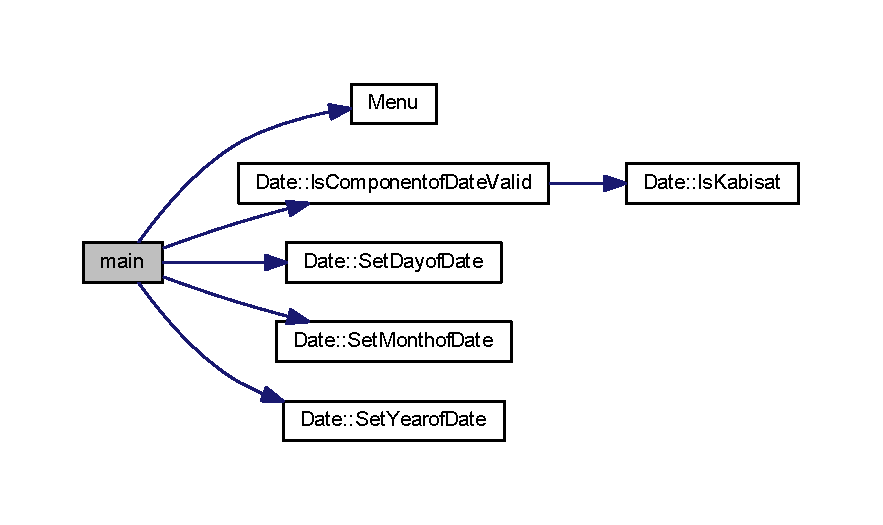
\includegraphics[width=350pt]{dc/d05/m_date_8cpp_ae66f6b31b5ad750f1fe042a706a4e3d4_cgraph}
\end{center}
\end{figure}


\hypertarget{m_date_8cpp_afdf1ca9e7afc3e7ec41b47fea4b3d80d}{\index{m\-Date.\-cpp@{m\-Date.\-cpp}!Menu@{Menu}}
\index{Menu@{Menu}!mDate.cpp@{m\-Date.\-cpp}}
\subsubsection[{Menu}]{\setlength{\rightskip}{0pt plus 5cm}void Menu (
\begin{DoxyParamCaption}
{}
\end{DoxyParamCaption}
)}}\label{m_date_8cpp_afdf1ca9e7afc3e7ec41b47fea4b3d80d}


Definition at line 83 of file m\-Date.\-cpp.



Here is the caller graph for this function\-:\nopagebreak
\begin{figure}[H]
\begin{center}
\leavevmode
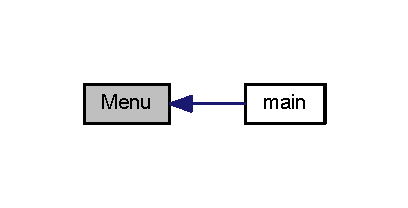
\includegraphics[width=196pt]{dc/d05/m_date_8cpp_afdf1ca9e7afc3e7ec41b47fea4b3d80d_icgraph}
\end{center}
\end{figure}



\hypertarget{_date_time_8cpp}{\section{Date\-Time/\-Date\-Time.cpp File Reference}
\label{_date_time_8cpp}\index{Date\-Time/\-Date\-Time.\-cpp@{Date\-Time/\-Date\-Time.\-cpp}}
}


Implementation \hyperlink{class_date_time}{Date\-Time} Class.  


{\ttfamily \#include \char`\"{}Date\-Time.\-h\char`\"{}}\\*
Include dependency graph for Date\-Time.\-cpp\-:\nopagebreak
\begin{figure}[H]
\begin{center}
\leavevmode
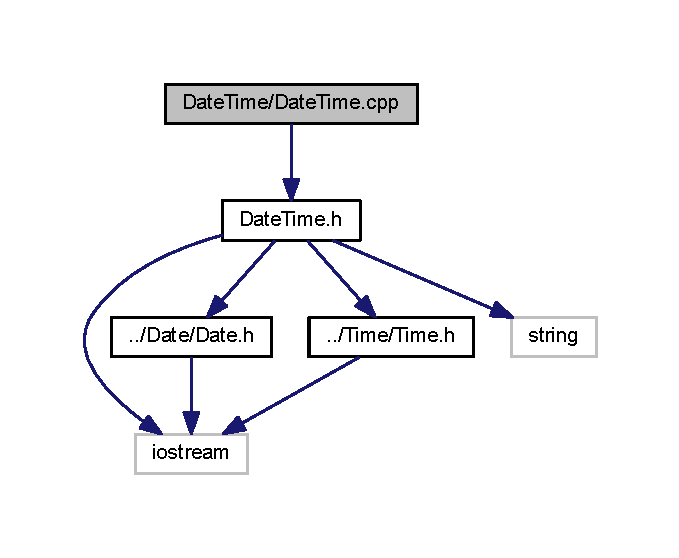
\includegraphics[width=326pt]{d1/dde/_date_time_8cpp__incl}
\end{center}
\end{figure}


\subsection{Detailed Description}
Implementation \hyperlink{class_date_time}{Date\-Time} Class. 

Definition in file \hyperlink{_date_time_8cpp_source}{Date\-Time.\-cpp}.


\hypertarget{_date_time_8h}{\section{Date\-Time/\-Date\-Time.h File Reference}
\label{_date_time_8h}\index{Date\-Time/\-Date\-Time.\-h@{Date\-Time/\-Date\-Time.\-h}}
}


Header \hyperlink{class_date_time}{Date\-Time} Class.  


{\ttfamily \#include $<$iostream$>$}\\*
{\ttfamily \#include \char`\"{}../\-Date/\-Date.\-h\char`\"{}}\\*
{\ttfamily \#include \char`\"{}../\-Time/\-Time.\-h\char`\"{}}\\*
{\ttfamily \#include $<$string$>$}\\*
Include dependency graph for Date\-Time.\-h\-:\nopagebreak
\begin{figure}[H]
\begin{center}
\leavevmode
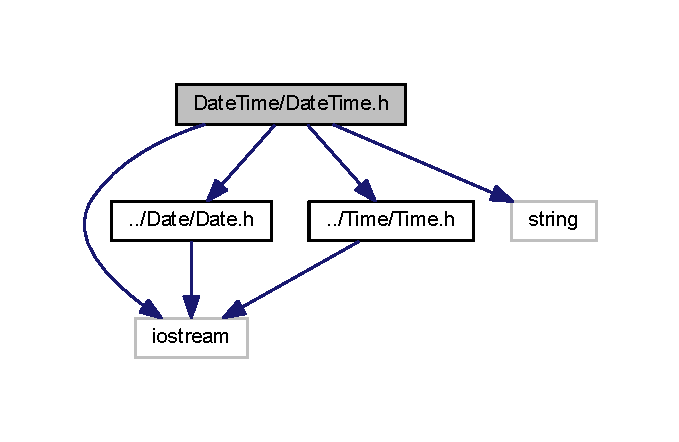
\includegraphics[width=326pt]{da/d28/_date_time_8h__incl}
\end{center}
\end{figure}
This graph shows which files directly or indirectly include this file\-:\nopagebreak
\begin{figure}[H]
\begin{center}
\leavevmode
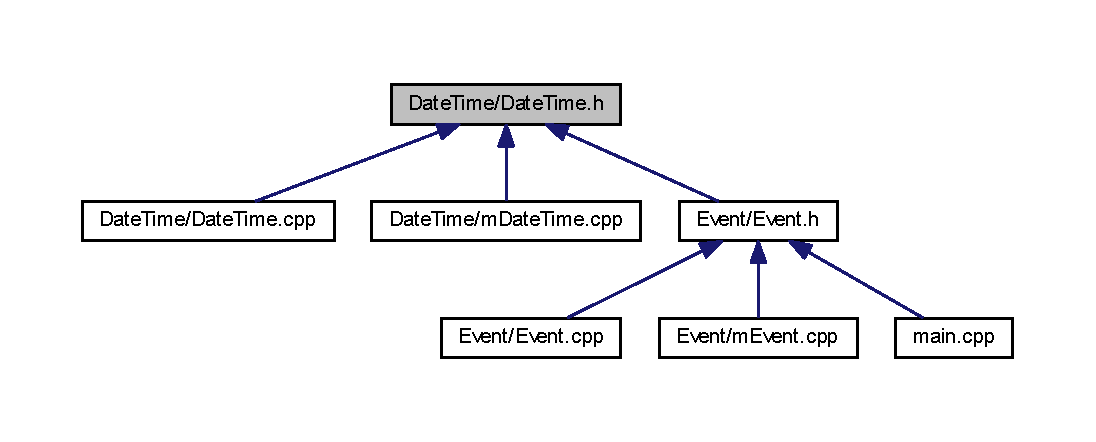
\includegraphics[width=350pt]{df/dcf/_date_time_8h__dep__incl}
\end{center}
\end{figure}
\subsection*{Classes}
\begin{DoxyCompactItemize}
\item 
class \hyperlink{class_date_time}{Date\-Time}
\begin{DoxyCompactList}\small\item\em \hyperlink{class_date_time}{Date\-Time} Class. \end{DoxyCompactList}\end{DoxyCompactItemize}


\subsection{Detailed Description}
Header \hyperlink{class_date_time}{Date\-Time} Class. 

Definition in file \hyperlink{_date_time_8h_source}{Date\-Time.\-h}.


\hypertarget{m_date_time_8cpp}{\section{Date\-Time/m\-Date\-Time.cpp File Reference}
\label{m_date_time_8cpp}\index{Date\-Time/m\-Date\-Time.\-cpp@{Date\-Time/m\-Date\-Time.\-cpp}}
}


Driver \hyperlink{class_date_time}{Date\-Time} Class.  


{\ttfamily \#include $<$iostream$>$}\\*
{\ttfamily \#include \char`\"{}Date\-Time.\-h\char`\"{}}\\*
Include dependency graph for m\-Date\-Time.\-cpp\-:\nopagebreak
\begin{figure}[H]
\begin{center}
\leavevmode
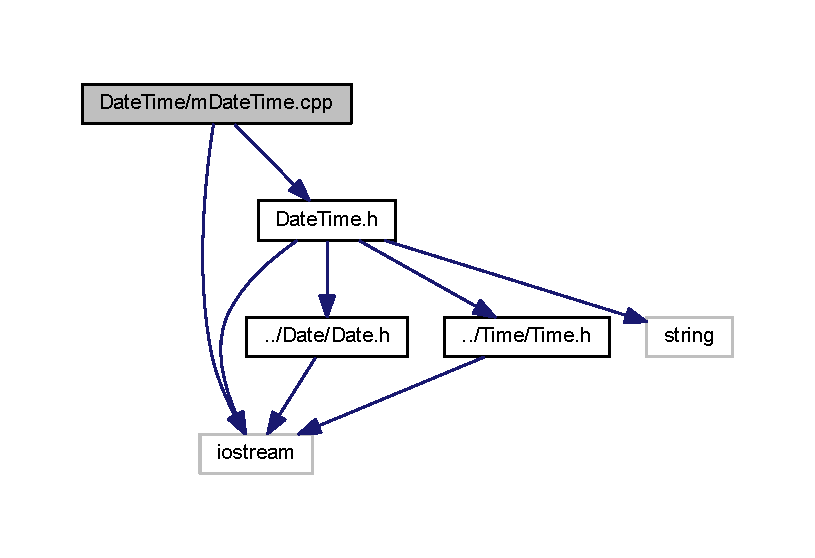
\includegraphics[width=350pt]{d6/de4/m_date_time_8cpp__incl}
\end{center}
\end{figure}
\subsection*{Functions}
\begin{DoxyCompactItemize}
\item 
void \hyperlink{m_date_time_8cpp_afdf1ca9e7afc3e7ec41b47fea4b3d80d}{Menu} ()
\item 
int \hyperlink{m_date_time_8cpp_ae66f6b31b5ad750f1fe042a706a4e3d4}{main} ()
\end{DoxyCompactItemize}


\subsection{Detailed Description}
Driver \hyperlink{class_date_time}{Date\-Time} Class. 

Definition in file \hyperlink{m_date_time_8cpp_source}{m\-Date\-Time.\-cpp}.



\subsection{Function Documentation}
\hypertarget{m_date_time_8cpp_ae66f6b31b5ad750f1fe042a706a4e3d4}{\index{m\-Date\-Time.\-cpp@{m\-Date\-Time.\-cpp}!main@{main}}
\index{main@{main}!mDateTime.cpp@{m\-Date\-Time.\-cpp}}
\subsubsection[{main}]{\setlength{\rightskip}{0pt plus 5cm}int main (
\begin{DoxyParamCaption}
{}
\end{DoxyParamCaption}
)}}\label{m_date_time_8cpp_ae66f6b31b5ad750f1fe042a706a4e3d4}


Definition at line 13 of file m\-Date\-Time.\-cpp.



Here is the call graph for this function\-:\nopagebreak
\begin{figure}[H]
\begin{center}
\leavevmode
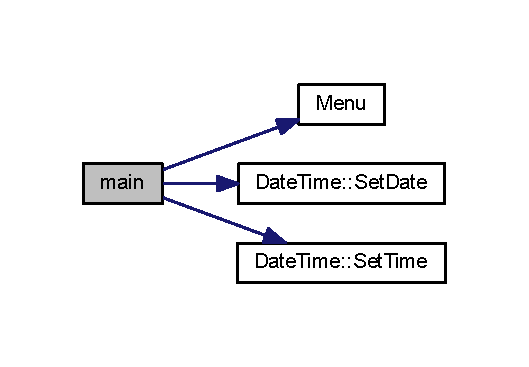
\includegraphics[width=254pt]{dc/d1f/m_date_time_8cpp_ae66f6b31b5ad750f1fe042a706a4e3d4_cgraph}
\end{center}
\end{figure}


\hypertarget{m_date_time_8cpp_afdf1ca9e7afc3e7ec41b47fea4b3d80d}{\index{m\-Date\-Time.\-cpp@{m\-Date\-Time.\-cpp}!Menu@{Menu}}
\index{Menu@{Menu}!mDateTime.cpp@{m\-Date\-Time.\-cpp}}
\subsubsection[{Menu}]{\setlength{\rightskip}{0pt plus 5cm}void Menu (
\begin{DoxyParamCaption}
{}
\end{DoxyParamCaption}
)}}\label{m_date_time_8cpp_afdf1ca9e7afc3e7ec41b47fea4b3d80d}


Definition at line 71 of file m\-Date\-Time.\-cpp.



Here is the caller graph for this function\-:\nopagebreak
\begin{figure}[H]
\begin{center}
\leavevmode
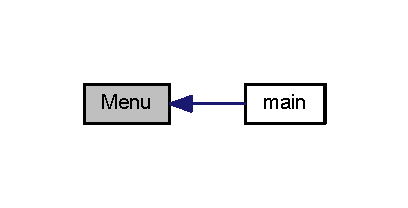
\includegraphics[width=196pt]{dc/d1f/m_date_time_8cpp_afdf1ca9e7afc3e7ec41b47fea4b3d80d_icgraph}
\end{center}
\end{figure}



\hypertarget{_event_8cpp}{\section{Event/\-Event.cpp File Reference}
\label{_event_8cpp}\index{Event/\-Event.\-cpp@{Event/\-Event.\-cpp}}
}


Implementation \hyperlink{class_event}{Event} Class.  


{\ttfamily \#include \char`\"{}Event.\-h\char`\"{}}\\*
Include dependency graph for Event.\-cpp\-:\nopagebreak
\begin{figure}[H]
\begin{center}
\leavevmode
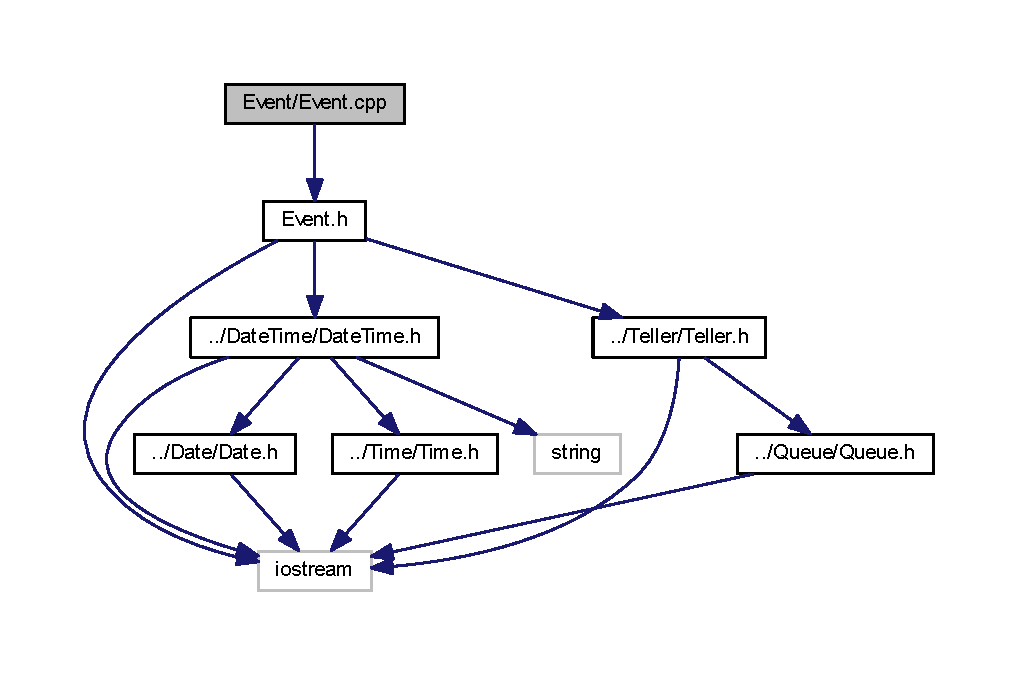
\includegraphics[width=350pt]{d9/d2e/_event_8cpp__incl}
\end{center}
\end{figure}


\subsection{Detailed Description}
Implementation \hyperlink{class_event}{Event} Class. 

Definition in file \hyperlink{_event_8cpp_source}{Event.\-cpp}.


\hypertarget{_event_8h}{\section{Event/\-Event.h File Reference}
\label{_event_8h}\index{Event/\-Event.\-h@{Event/\-Event.\-h}}
}


Header \hyperlink{class_event}{Event} Class.  


{\ttfamily \#include $<$iostream$>$}\\*
{\ttfamily \#include \char`\"{}../\-Date\-Time/\-Date\-Time.\-h\char`\"{}}\\*
{\ttfamily \#include \char`\"{}../\-Teller/\-Teller.\-h\char`\"{}}\\*
Include dependency graph for Event.\-h\-:\nopagebreak
\begin{figure}[H]
\begin{center}
\leavevmode
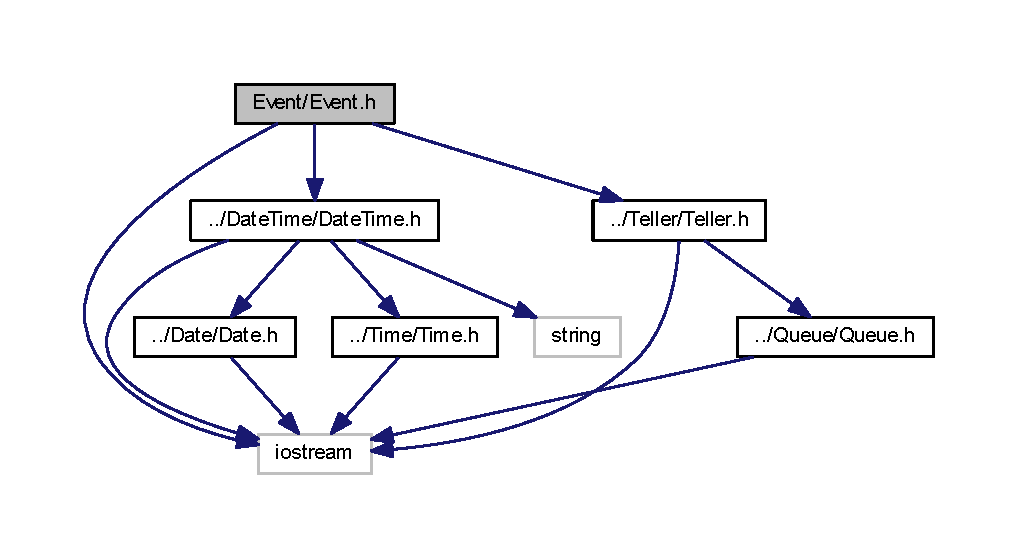
\includegraphics[width=350pt]{d3/d46/_event_8h__incl}
\end{center}
\end{figure}
This graph shows which files directly or indirectly include this file\-:\nopagebreak
\begin{figure}[H]
\begin{center}
\leavevmode
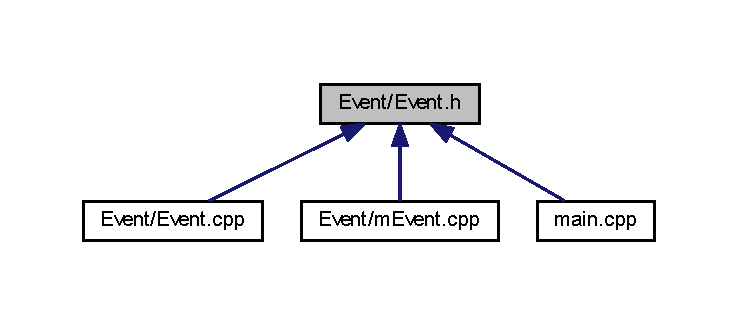
\includegraphics[width=350pt]{d7/daa/_event_8h__dep__incl}
\end{center}
\end{figure}
\subsection*{Classes}
\begin{DoxyCompactItemize}
\item 
class \hyperlink{class_event}{Event}
\begin{DoxyCompactList}\small\item\em \hyperlink{class_event}{Event} Class. \end{DoxyCompactList}\end{DoxyCompactItemize}


\subsection{Detailed Description}
Header \hyperlink{class_event}{Event} Class. 

Definition in file \hyperlink{_event_8h_source}{Event.\-h}.


\hypertarget{m_event_8cpp}{\section{Event/m\-Event.cpp File Reference}
\label{m_event_8cpp}\index{Event/m\-Event.\-cpp@{Event/m\-Event.\-cpp}}
}


Driver \hyperlink{class_event}{Event} Class.  


{\ttfamily \#include $<$iostream$>$}\\*
{\ttfamily \#include \char`\"{}Event.\-h\char`\"{}}\\*
Include dependency graph for m\-Event.\-cpp\-:\nopagebreak
\begin{figure}[H]
\begin{center}
\leavevmode
\includegraphics[width=350pt]{d6/d95/m_event_8cpp__incl}
\end{center}
\end{figure}
\subsection*{Functions}
\begin{DoxyCompactItemize}
\item 
int \hyperlink{m_event_8cpp_ae66f6b31b5ad750f1fe042a706a4e3d4}{main} ()
\end{DoxyCompactItemize}


\subsection{Detailed Description}
Driver \hyperlink{class_event}{Event} Class. 

Definition in file \hyperlink{m_event_8cpp_source}{m\-Event.\-cpp}.



\subsection{Function Documentation}
\hypertarget{m_event_8cpp_ae66f6b31b5ad750f1fe042a706a4e3d4}{\index{m\-Event.\-cpp@{m\-Event.\-cpp}!main@{main}}
\index{main@{main}!mEvent.cpp@{m\-Event.\-cpp}}
\subsubsection[{main}]{\setlength{\rightskip}{0pt plus 5cm}int main (
\begin{DoxyParamCaption}
{}
\end{DoxyParamCaption}
)}}\label{m_event_8cpp_ae66f6b31b5ad750f1fe042a706a4e3d4}


Definition at line 11 of file m\-Event.\-cpp.



Here is the call graph for this function\-:\nopagebreak
\begin{figure}[H]
\begin{center}
\leavevmode
\includegraphics[width=350pt]{d2/dd2/m_event_8cpp_ae66f6b31b5ad750f1fe042a706a4e3d4_cgraph}
\end{center}
\end{figure}



\hypertarget{main_8cpp}{\section{main.\-cpp File Reference}
\label{main_8cpp}\index{main.\-cpp@{main.\-cpp}}
}


Main Program of All Classes.  


{\ttfamily \#include $<$iostream$>$}\\*
{\ttfamily \#include \char`\"{}Event/\-Event.\-h\char`\"{}}\\*
Include dependency graph for main.\-cpp\-:\nopagebreak
\begin{figure}[H]
\begin{center}
\leavevmode
\includegraphics[width=350pt]{da/dce/main_8cpp__incl}
\end{center}
\end{figure}
\subsection*{Functions}
\begin{DoxyCompactItemize}
\item 
int \hyperlink{main_8cpp_ae66f6b31b5ad750f1fe042a706a4e3d4}{main} ()
\end{DoxyCompactItemize}


\subsection{Detailed Description}
Main Program of All Classes. 

Definition in file \hyperlink{main_8cpp_source}{main.\-cpp}.



\subsection{Function Documentation}
\hypertarget{main_8cpp_ae66f6b31b5ad750f1fe042a706a4e3d4}{\index{main.\-cpp@{main.\-cpp}!main@{main}}
\index{main@{main}!main.cpp@{main.\-cpp}}
\subsubsection[{main}]{\setlength{\rightskip}{0pt plus 5cm}int main (
\begin{DoxyParamCaption}
{}
\end{DoxyParamCaption}
)}}\label{main_8cpp_ae66f6b31b5ad750f1fe042a706a4e3d4}


Definition at line 11 of file main.\-cpp.



Here is the call graph for this function\-:\nopagebreak
\begin{figure}[H]
\begin{center}
\leavevmode
\includegraphics[width=350pt]{df/d0a/main_8cpp_ae66f6b31b5ad750f1fe042a706a4e3d4_cgraph}
\end{center}
\end{figure}



\hypertarget{m_queue_8cpp}{\section{Queue/m\-Queue.cpp File Reference}
\label{m_queue_8cpp}\index{Queue/m\-Queue.\-cpp@{Queue/m\-Queue.\-cpp}}
}


Driver \hyperlink{class_queue}{Queue} Class.  


{\ttfamily \#include \char`\"{}Queue.\-h\char`\"{}}\\*
{\ttfamily \#include $<$iostream$>$}\\*
Include dependency graph for m\-Queue.\-cpp\-:\nopagebreak
\begin{figure}[H]
\begin{center}
\leavevmode
\includegraphics[width=185pt]{d4/da3/m_queue_8cpp__incl}
\end{center}
\end{figure}
\subsection*{Functions}
\begin{DoxyCompactItemize}
\item 
void \hyperlink{m_queue_8cpp_afdf1ca9e7afc3e7ec41b47fea4b3d80d}{Menu} ()
\item 
int \hyperlink{m_queue_8cpp_ae66f6b31b5ad750f1fe042a706a4e3d4}{main} ()
\end{DoxyCompactItemize}


\subsection{Detailed Description}
Driver \hyperlink{class_queue}{Queue} Class. 

Definition in file \hyperlink{m_queue_8cpp_source}{m\-Queue.\-cpp}.



\subsection{Function Documentation}
\hypertarget{m_queue_8cpp_ae66f6b31b5ad750f1fe042a706a4e3d4}{\index{m\-Queue.\-cpp@{m\-Queue.\-cpp}!main@{main}}
\index{main@{main}!mQueue.cpp@{m\-Queue.\-cpp}}
\subsubsection[{main}]{\setlength{\rightskip}{0pt plus 5cm}int main (
\begin{DoxyParamCaption}
{}
\end{DoxyParamCaption}
)}}\label{m_queue_8cpp_ae66f6b31b5ad750f1fe042a706a4e3d4}


Definition at line 13 of file m\-Queue.\-cpp.



Here is the call graph for this function\-:\nopagebreak
\begin{figure}[H]
\begin{center}
\leavevmode
\includegraphics[width=350pt]{d5/df3/m_queue_8cpp_ae66f6b31b5ad750f1fe042a706a4e3d4_cgraph}
\end{center}
\end{figure}


\hypertarget{m_queue_8cpp_afdf1ca9e7afc3e7ec41b47fea4b3d80d}{\index{m\-Queue.\-cpp@{m\-Queue.\-cpp}!Menu@{Menu}}
\index{Menu@{Menu}!mQueue.cpp@{m\-Queue.\-cpp}}
\subsubsection[{Menu}]{\setlength{\rightskip}{0pt plus 5cm}void Menu (
\begin{DoxyParamCaption}
{}
\end{DoxyParamCaption}
)}}\label{m_queue_8cpp_afdf1ca9e7afc3e7ec41b47fea4b3d80d}


Definition at line 60 of file m\-Queue.\-cpp.



Here is the caller graph for this function\-:\nopagebreak
\begin{figure}[H]
\begin{center}
\leavevmode
\includegraphics[width=196pt]{d5/df3/m_queue_8cpp_afdf1ca9e7afc3e7ec41b47fea4b3d80d_icgraph}
\end{center}
\end{figure}



\hypertarget{_queue_8cpp}{\section{Queue/\-Queue.cpp File Reference}
\label{_queue_8cpp}\index{Queue/\-Queue.\-cpp@{Queue/\-Queue.\-cpp}}
}


Implementation \hyperlink{class_queue}{Queue} Class.  


{\ttfamily \#include \char`\"{}Queue.\-h\char`\"{}}\\*
{\ttfamily \#include $<$cstdlib$>$}\\*
Include dependency graph for Queue.\-cpp\-:\nopagebreak
\begin{figure}[H]
\begin{center}
\leavevmode
\includegraphics[width=196pt]{d3/d91/_queue_8cpp__incl}
\end{center}
\end{figure}


\subsection{Detailed Description}
Implementation \hyperlink{class_queue}{Queue} Class. 

Definition in file \hyperlink{_queue_8cpp_source}{Queue.\-cpp}.


\hypertarget{_queue_8h}{\section{Queue/\-Queue.h File Reference}
\label{_queue_8h}\index{Queue/\-Queue.\-h@{Queue/\-Queue.\-h}}
}


Header \hyperlink{class_queue}{Queue} Class.  


{\ttfamily \#include $<$iostream$>$}\\*
Include dependency graph for Queue.\-h\-:\nopagebreak
\begin{figure}[H]
\begin{center}
\leavevmode
\includegraphics[width=164pt]{dd/d41/_queue_8h__incl}
\end{center}
\end{figure}
This graph shows which files directly or indirectly include this file\-:\nopagebreak
\begin{figure}[H]
\begin{center}
\leavevmode
\includegraphics[width=350pt]{d4/daa/_queue_8h__dep__incl}
\end{center}
\end{figure}
\subsection*{Classes}
\begin{DoxyCompactItemize}
\item 
class \hyperlink{class_queue}{Queue}
\begin{DoxyCompactList}\small\item\em \hyperlink{class_queue}{Queue} Class. \end{DoxyCompactList}\end{DoxyCompactItemize}


\subsection{Detailed Description}
Header \hyperlink{class_queue}{Queue} Class. 

Definition in file \hyperlink{_queue_8h_source}{Queue.\-h}.


\hypertarget{_r_e_a_d_m_e_8md}{\section{R\-E\-A\-D\-M\-E.\-md File Reference}
\label{_r_e_a_d_m_e_8md}\index{R\-E\-A\-D\-M\-E.\-md@{R\-E\-A\-D\-M\-E.\-md}}
}

\hypertarget{m_teller_8cpp}{\section{Teller/m\-Teller.cpp File Reference}
\label{m_teller_8cpp}\index{Teller/m\-Teller.\-cpp@{Teller/m\-Teller.\-cpp}}
}


Driver \hyperlink{class_teller}{Teller} Class.  


{\ttfamily \#include \char`\"{}Teller.\-h\char`\"{}}\\*
{\ttfamily \#include $<$iostream$>$}\\*
{\ttfamily \#include $<$string$>$}\\*
Include dependency graph for m\-Teller.\-cpp\-:\nopagebreak
\begin{figure}[H]
\begin{center}
\leavevmode
\includegraphics[width=309pt]{df/d7e/m_teller_8cpp__incl}
\end{center}
\end{figure}
\subsection*{Functions}
\begin{DoxyCompactItemize}
\item 
int \hyperlink{m_teller_8cpp_ae66f6b31b5ad750f1fe042a706a4e3d4}{main} ()
\end{DoxyCompactItemize}


\subsection{Detailed Description}
Driver \hyperlink{class_teller}{Teller} Class. 

Definition in file \hyperlink{m_teller_8cpp_source}{m\-Teller.\-cpp}.



\subsection{Function Documentation}
\hypertarget{m_teller_8cpp_ae66f6b31b5ad750f1fe042a706a4e3d4}{\index{m\-Teller.\-cpp@{m\-Teller.\-cpp}!main@{main}}
\index{main@{main}!mTeller.cpp@{m\-Teller.\-cpp}}
\subsubsection[{main}]{\setlength{\rightskip}{0pt plus 5cm}int main (
\begin{DoxyParamCaption}
{}
\end{DoxyParamCaption}
)}}\label{m_teller_8cpp_ae66f6b31b5ad750f1fe042a706a4e3d4}


Definition at line 12 of file m\-Teller.\-cpp.



Here is the call graph for this function\-:\nopagebreak
\begin{figure}[H]
\begin{center}
\leavevmode
\includegraphics[width=350pt]{d6/dea/m_teller_8cpp_ae66f6b31b5ad750f1fe042a706a4e3d4_cgraph}
\end{center}
\end{figure}



\hypertarget{_teller_8cpp}{\section{Teller/\-Teller.cpp File Reference}
\label{_teller_8cpp}\index{Teller/\-Teller.\-cpp@{Teller/\-Teller.\-cpp}}
}


Implementation \hyperlink{class_teller}{Teller} Class.  


{\ttfamily \#include $<$cmath$>$}\\*
{\ttfamily \#include \char`\"{}Teller.\-h\char`\"{}}\\*
Include dependency graph for Teller.\-cpp\-:\nopagebreak
\begin{figure}[H]
\begin{center}
\leavevmode
\includegraphics[width=192pt]{d3/dbc/_teller_8cpp__incl}
\end{center}
\end{figure}


\subsection{Detailed Description}
Implementation \hyperlink{class_teller}{Teller} Class. 

Definition in file \hyperlink{_teller_8cpp_source}{Teller.\-cpp}.


\hypertarget{_teller_8h}{\section{Teller/\-Teller.h File Reference}
\label{_teller_8h}\index{Teller/\-Teller.\-h@{Teller/\-Teller.\-h}}
}


Header \hyperlink{class_teller}{Teller} Class.  


{\ttfamily \#include \char`\"{}../\-Queue/\-Queue.\-h\char`\"{}}\\*
{\ttfamily \#include $<$iostream$>$}\\*
Include dependency graph for Teller.\-h\-:\nopagebreak
\begin{figure}[H]
\begin{center}
\leavevmode
\includegraphics[width=201pt]{d7/dba/_teller_8h__incl}
\end{center}
\end{figure}
This graph shows which files directly or indirectly include this file\-:\nopagebreak
\begin{figure}[H]
\begin{center}
\leavevmode
\includegraphics[width=350pt]{d9/d2c/_teller_8h__dep__incl}
\end{center}
\end{figure}
\subsection*{Classes}
\begin{DoxyCompactItemize}
\item 
class \hyperlink{class_teller}{Teller}
\begin{DoxyCompactList}\small\item\em \hyperlink{class_teller}{Teller} Class. \end{DoxyCompactList}\end{DoxyCompactItemize}


\subsection{Detailed Description}
Header \hyperlink{class_teller}{Teller} Class. 

Definition in file \hyperlink{_teller_8h_source}{Teller.\-h}.


\hypertarget{m_time_8cpp}{\section{Time/m\-Time.cpp File Reference}
\label{m_time_8cpp}\index{Time/m\-Time.\-cpp@{Time/m\-Time.\-cpp}}
}


Driver \hyperlink{class_time}{Time} Class.  


{\ttfamily \#include $<$iostream$>$}\\*
{\ttfamily \#include \char`\"{}Time.\-h\char`\"{}}\\*
Include dependency graph for m\-Time.\-cpp\-:\nopagebreak
\begin{figure}[H]
\begin{center}
\leavevmode
\includegraphics[width=173pt]{df/d41/m_time_8cpp__incl}
\end{center}
\end{figure}
\subsection*{Functions}
\begin{DoxyCompactItemize}
\item 
void \hyperlink{m_time_8cpp_afdf1ca9e7afc3e7ec41b47fea4b3d80d}{Menu} ()
\item 
int \hyperlink{m_time_8cpp_ae66f6b31b5ad750f1fe042a706a4e3d4}{main} ()
\end{DoxyCompactItemize}


\subsection{Detailed Description}
Driver \hyperlink{class_time}{Time} Class. 

Definition in file \hyperlink{m_time_8cpp_source}{m\-Time.\-cpp}.



\subsection{Function Documentation}
\hypertarget{m_time_8cpp_ae66f6b31b5ad750f1fe042a706a4e3d4}{\index{m\-Time.\-cpp@{m\-Time.\-cpp}!main@{main}}
\index{main@{main}!mTime.cpp@{m\-Time.\-cpp}}
\subsubsection[{main}]{\setlength{\rightskip}{0pt plus 5cm}int main (
\begin{DoxyParamCaption}
{}
\end{DoxyParamCaption}
)}}\label{m_time_8cpp_ae66f6b31b5ad750f1fe042a706a4e3d4}


Definition at line 13 of file m\-Time.\-cpp.



Here is the call graph for this function\-:\nopagebreak
\begin{figure}[H]
\begin{center}
\leavevmode
\includegraphics[width=292pt]{da/db2/m_time_8cpp_ae66f6b31b5ad750f1fe042a706a4e3d4_cgraph}
\end{center}
\end{figure}


\hypertarget{m_time_8cpp_afdf1ca9e7afc3e7ec41b47fea4b3d80d}{\index{m\-Time.\-cpp@{m\-Time.\-cpp}!Menu@{Menu}}
\index{Menu@{Menu}!mTime.cpp@{m\-Time.\-cpp}}
\subsubsection[{Menu}]{\setlength{\rightskip}{0pt plus 5cm}void Menu (
\begin{DoxyParamCaption}
{}
\end{DoxyParamCaption}
)}}\label{m_time_8cpp_afdf1ca9e7afc3e7ec41b47fea4b3d80d}


Definition at line 81 of file m\-Time.\-cpp.



Here is the caller graph for this function\-:\nopagebreak
\begin{figure}[H]
\begin{center}
\leavevmode
\includegraphics[width=196pt]{da/db2/m_time_8cpp_afdf1ca9e7afc3e7ec41b47fea4b3d80d_icgraph}
\end{center}
\end{figure}



\hypertarget{_time_8cpp}{\section{Time/\-Time.cpp File Reference}
\label{_time_8cpp}\index{Time/\-Time.\-cpp@{Time/\-Time.\-cpp}}
}


Implementation \hyperlink{class_time}{Time} Class.  


{\ttfamily \#include \char`\"{}Time.\-h\char`\"{}}\\*
Include dependency graph for Time.\-cpp\-:\nopagebreak
\begin{figure}[H]
\begin{center}
\leavevmode
\includegraphics[width=160pt]{d1/db0/_time_8cpp__incl}
\end{center}
\end{figure}


\subsection{Detailed Description}
Implementation \hyperlink{class_time}{Time} Class. 

Definition in file \hyperlink{_time_8cpp_source}{Time.\-cpp}.


\hypertarget{_time_8h}{\section{Time/\-Time.h File Reference}
\label{_time_8h}\index{Time/\-Time.\-h@{Time/\-Time.\-h}}
}


Header \hyperlink{class_time}{Time} Class.  


{\ttfamily \#include $<$iostream$>$}\\*
Include dependency graph for Time.\-h\-:\nopagebreak
\begin{figure}[H]
\begin{center}
\leavevmode
\includegraphics[width=150pt]{dc/d6d/_time_8h__incl}
\end{center}
\end{figure}
This graph shows which files directly or indirectly include this file\-:\nopagebreak
\begin{figure}[H]
\begin{center}
\leavevmode
\includegraphics[width=350pt]{db/db1/_time_8h__dep__incl}
\end{center}
\end{figure}
\subsection*{Classes}
\begin{DoxyCompactItemize}
\item 
class \hyperlink{class_time}{Time}
\begin{DoxyCompactList}\small\item\em \hyperlink{class_time}{Time} Class. \end{DoxyCompactList}\end{DoxyCompactItemize}


\subsection{Detailed Description}
Header \hyperlink{class_time}{Time} Class. 

Definition in file \hyperlink{_time_8h_source}{Time.\-h}.


%--- End generated contents ---

% Index
\newpage
\phantomsection
\addcontentsline{toc}{chapter}{Index}
\printindex

\end{document}
